\documentclass[12pt]{article}

\usepackage{amssymb}
\usepackage{amsmath}
\usepackage{bm}
\usepackage{dsfont}
\usepackage[margin=1in]{geometry}
\usepackage[font=scriptsize]{caption}
\usepackage{dsfont}
\usepackage{amsmath}
\usepackage{graphicx}
\usepackage{bm}
\newcommand{\m}[1]{\mathbf{\bm{#1}}}
\newcommand{\R}{I\hspace{-4.4pt}R}
\newcommand{\bc}[1]{\textcolor{blue}{\mathbf{#1}}}
\newcommand{\ind}{\mathds{1}}
\newcommand{\m}[1]{\mathbf{\bm{#1}}}
\newcommand{\R}{I\hspace{-4.4pt}R}

% \setlength\parindent{0pt}


\begin{document}

\begin{Large}
\noindent Extreme value comparison of climate simulations and observations
\end{Large}
% A Bayesian hierarchical model for CanCM4 climate simulations, with an exploration of estimating the extremal index in the hierarchical setting, and a comparison between climate simulations and observations from a gridded product

\section{Abstract}

We propose a hierarchical extension to univariate extreme value modeling. In the univariate setting it is common to work with a single time-series or spatial field. However, having multiple realizations from computer simulations at a variety of input settings suggests an extension to a hierarchical formulation. The extremal index $\theta$, in turn, is estimated hierarchically, requiring an adjustment to the declustering scheme. The hierarchical model is fit to climate data.

\section{Introduction}



Extreme value theory provides the framework for analyzing the stochastic behavior of a process at very large (small) values. This entails calculating the probability distribution of the maximum (minimum) of a sequence of random variabes. 

Equivalently, extreme value analyses study the tails of probability distributions associated with some data generating mechanism. 

In extreme value analyses, a primary interest is to understand 

The standard approach is to appeal to asymtoptic arguments.

We can calculate useful quantities such as return levels.

This allows us to extrapolate beyond the span of historical data.


We compare three types of climate model simulations 

The Fourth Generation Atmospheric General Circulation Model (CanCM4) from Canada 

Decadal, historical, and control runs are used to obtain precipitation and temperature over California and the U.S. We have observational data from Ed Maurer. We will consider two 10-year periods: 1962--1971 and 1990--1999. We will also split these into winter months (December, January, Februrary) and summer months (June, July, August). Precipitation in summer is not analyzed.
\bigskip

Purpose of the univariate analysis?
\bigskip

Details on the differences between decadal, historical, and control runs.
\bigskip

Precipitation based on the observations is summed. Precipitation from the climate model is computed with a weighted sum, based on the number of locations in the observation product.
\bigskip

Description of data processing
\bigskip

Picture of the locations CanCM4/Obs produces
\bigskip

Time-series plot of the variables
\bigskip

\begin{figure}
\begin{center}
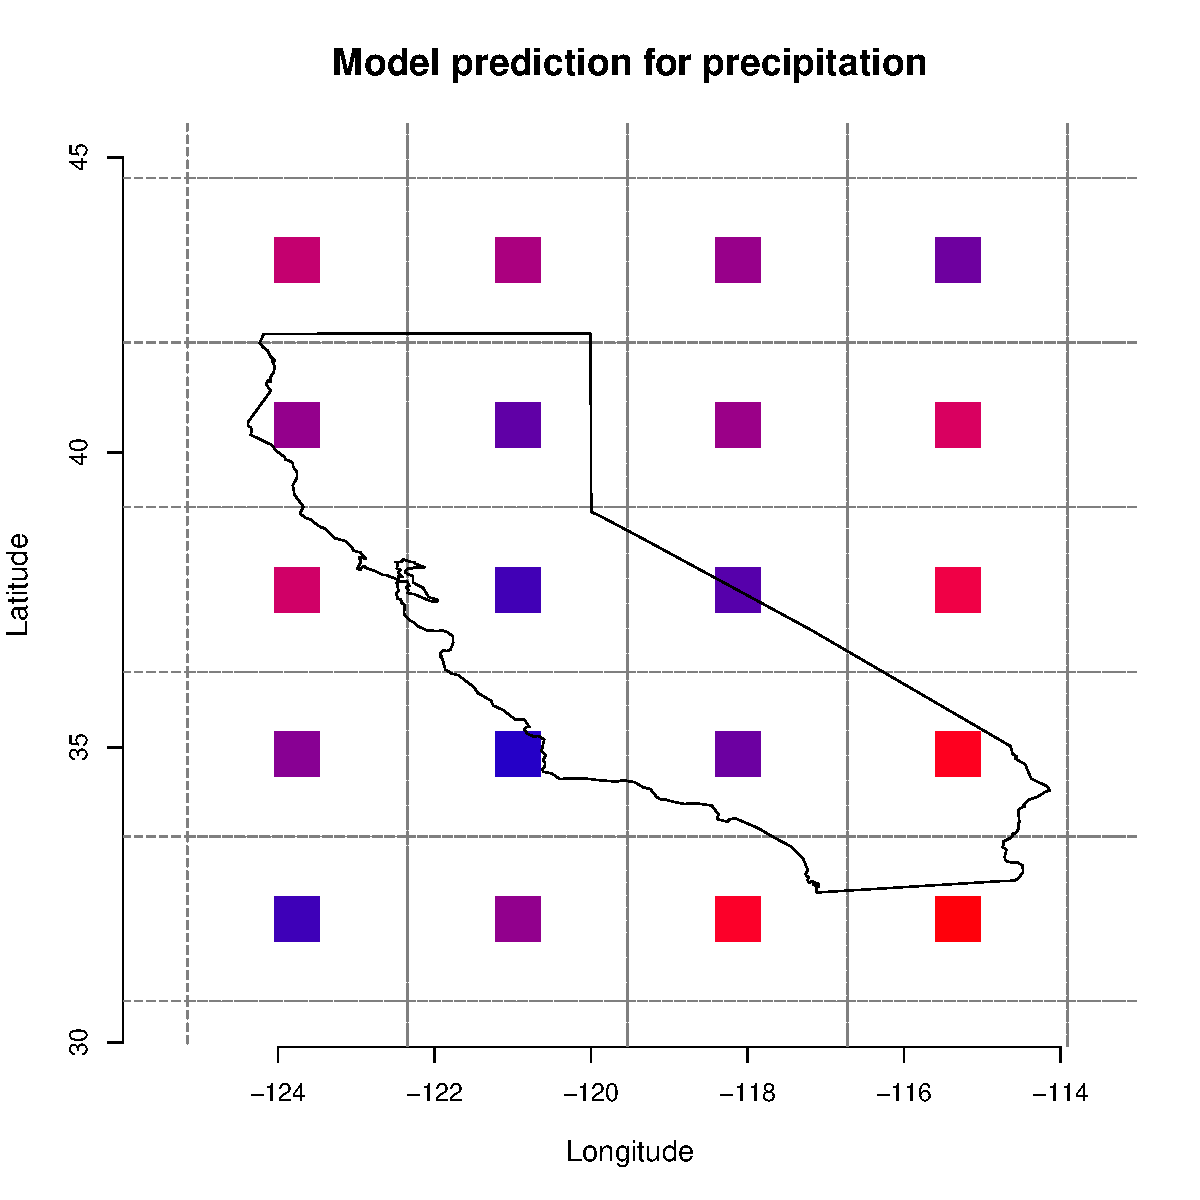
\includegraphics[scale=0.26]{/home/mickey/files/repos/stat_clim_evt_repo/figs/cal_mod_box1.pdf}
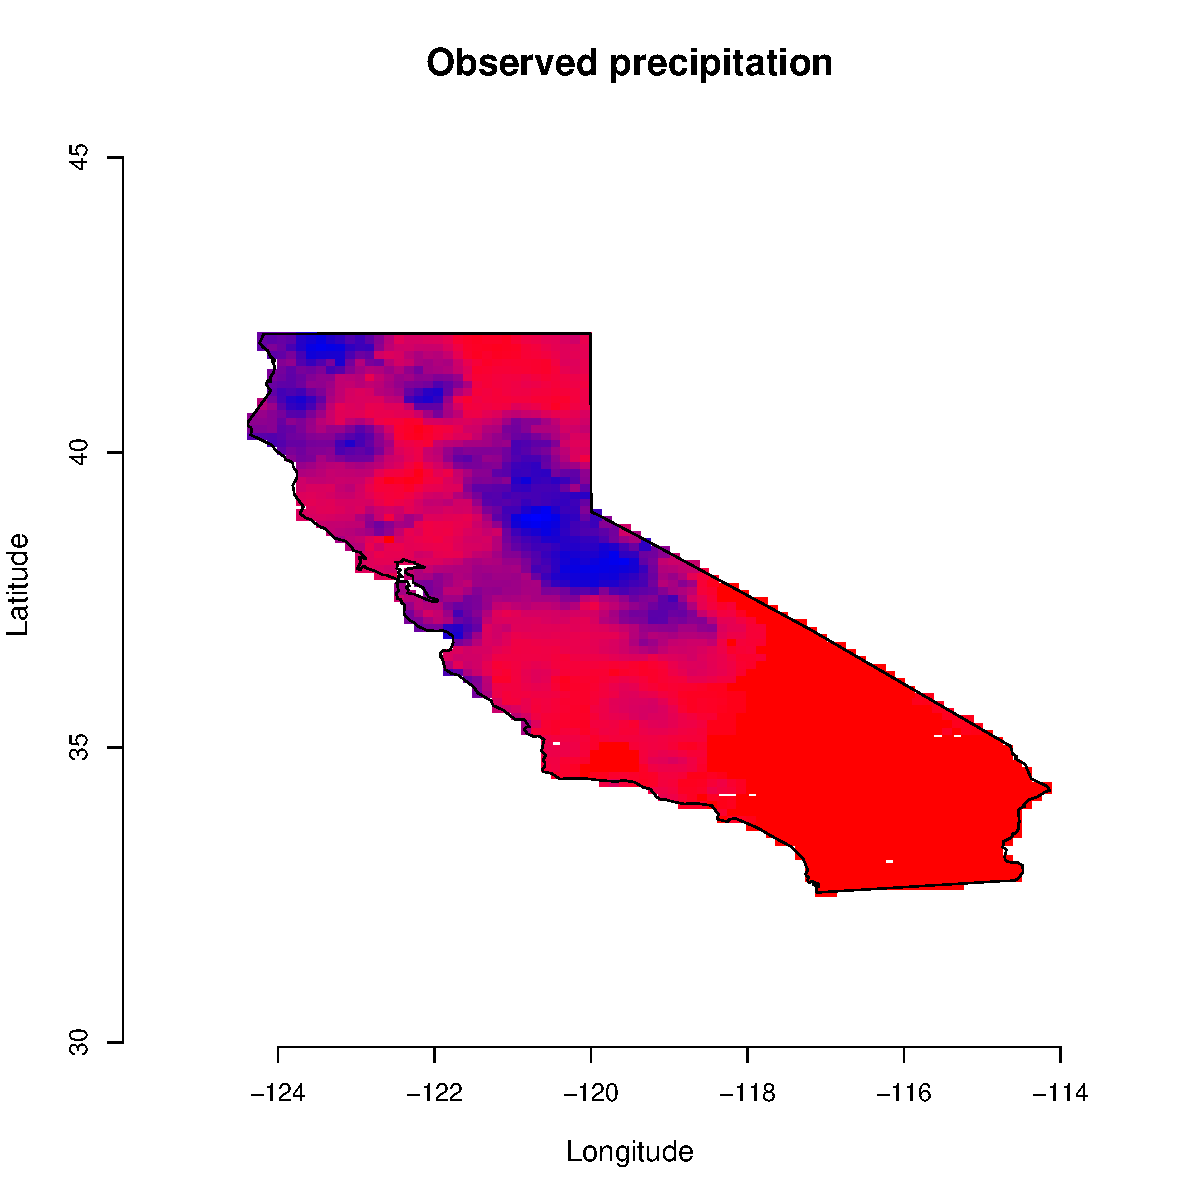
\includegraphics[scale=0.26]{/home/mickey/files/repos/stat_clim_evt_repo/figs/cal_mod_box2.pdf}
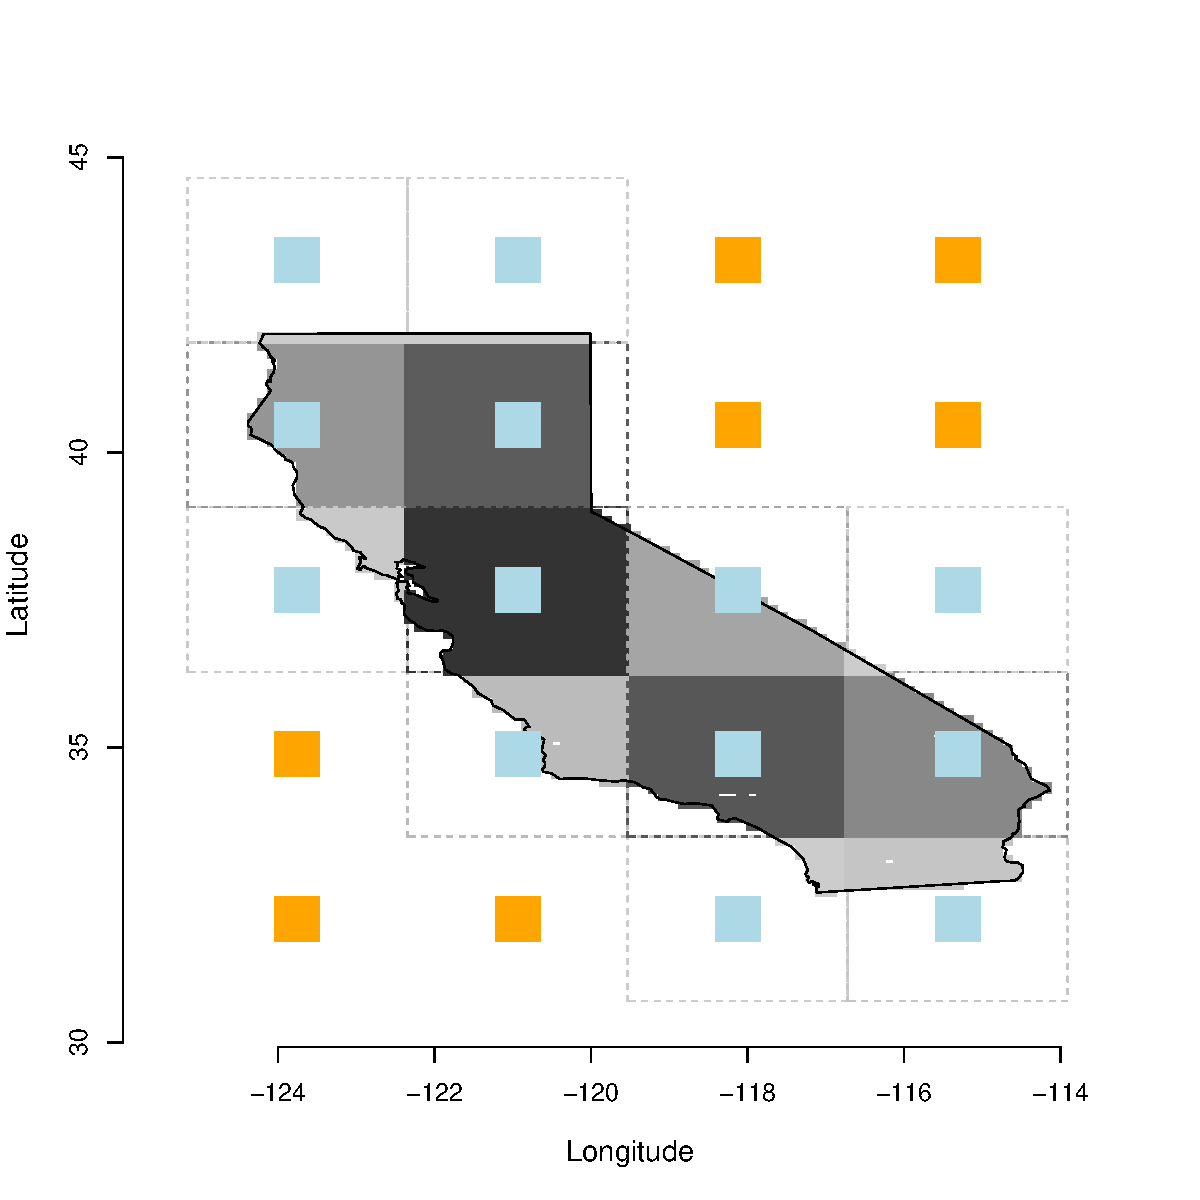
\includegraphics[scale=0.26]{/home/mickey/files/repos/stat_clim_evt_repo/figs/cal_mod_box3.pdf}
\end{center}
\caption{Left: CanCM4 simulation locations. Center: Observation locations. Right: method for computing weighted sum or average for CanCM4 to make values comparable with observations.}
\end{figure}
 
\section{Threshold exceedance model}

A threshold exceedance model considers observations from a random variable $X$ that are greater than some large threshold $u$. If the distribution of $X$, $F_X$, is known, then we can compute the distribution of the exceedances $Y=X-u$. For $y>0$,
\begin{align}
P(X-u\leq y| X > u) = 1-\frac{1-F_X(y+u)}{1-F_X(u)}.
\end{align}
% \begin{align}
% P(X-u\leq y| X > u) &= 1-P(X-u>y|X>u) = 1-\frac{P(X>u+y, X>u)}{P(X>u)} \nonumber \\
%  &= 1-\frac{P(X>y+u)}{P(X>u)} = 1-\frac{1-F_X(y+u)}{1-F_X(u)}.
% \end{align}

When $F_X$ is not known, a standard approach is to approximate (1) with the generalized Pareto distribution (see Theorem 4.1 of Coles (2001) page 75). The following is a summary of the theorem.
\bigskip

Let $X_1,X_2,\ldots$ be a sequence of independent random variables with common distribution. Then for large enough $u$, the distribution of $(X-u)$, conditional on $X>u$ is approximately
\begin{align}
P(X-u\leq y|X>u) \approx H(y) = 1 - \left(1+\frac{\xi y}{\sigma}\right)^{-1/\xi} \label{gpapprox}
\end{align}
defined on $\{y:y>0~\mathrm{and}~(1+\xi y/\sigma) >0\}$. $H(y)$ is the distribution function for a generalized Pareto random variable with parameters $\sigma>0$ and $\xi$.
\bigskip

For excesses $y_1,\ldots,y_k$ of a threshold $u$, the likelihood of $(\sigma,\xi)$ is derived from (\ref{gpapprox}) as
\begin{align}
L(y_1,\ldots,y_k;\sigma,\xi)=\sigma^{-k}\sum_{i=1}^k\left(1+\frac{\xi y_i}{\sigma}\right)_+^{-1/\xi-1}
\end{align}
where $z_+=\max(z,0)$. In many cases, the assumption of independence in observations may be too strong. When we have dependent random variables, which is likely the case in a time series, we employ a declustering scheme to obtain independent clusters (see Section 5).
\bigskip

% \begin{align*}
% P(X-u\leq y|X > u) &= P(X\leq y+u|X > u) \\
%  &= 1 - P(X> y+u|X > u) \\
%  &= 1 - \frac{P(X>y+u, X>u)}{P(X>u)}  \\
%  &= 1 - \frac{P(X>y+u)}{P(X>u)}  \\
%  &= 1 - \frac{1-P(X-u \leq y)}{P(X>u)}  \\
% \Rightarrow P(Y\leq y) = P(X-u\leq y) &= 1-P(X>u)\left(1 - P(X-u\leq y|X>u)\right) \\
%  &= 1-\zeta\left(1+\frac{\xi y}{\sigma}\right)^{-1/xi} \\
% \end{align*}
% where $\zeta=P(X>u)$.
% \bigskip

\subsection{Hierarchical model}

To extend this to the hierarchical setting, suppose we have $R$ replicates or computer simulations, each with $n_i$ observations, for $i=1,\ldots,R$. Let $X_{ij}$ denote the $j$th observation in replicate $i$. We assume
\[ X_{ij} \sim F_i,~~~~~i=1,\ldots,R,~~~~~j=1,\ldots,n_i \]
and all $X_{ij}$ are mutually conditionally independent. For a fixed $u$ and each $i$, define the following sets:
\[ A_i = \{j:x_{ij}\leq u\},~~~ A_i^c = \{j: x_{ij}>u\} \]
where $|A_i|=n_i-k_i$ and $|A_i^c|=k_i$ with $k_i$ being the number of exceedances in replicate $i$. We define our exceedances as
\[ y_{ij} = (x_{ij}-u)\cdot \ind_{(j \in A_i^c)} \]
so that all observations not exceeding $u$ are marked as $0$. Let $\m{y}_i=(y_{i,1},\ldots,y_{i,n_i})^\top$ and $\m{y}=(\m{y}_1^\top,\ldots,\m{y}_R^\top)^\top$.
\bigskip

\noindent The likelihood is given by
\begin{eqnarray*}
L(\m{y}; \m{\sigma}, \m{\xi}, \m{\zeta}) &=& \prod_{i=1}^R f_{Y_i}(\m{y}_i|\sigma_i,\xi_i,\zeta_i) \\
&=& \prod_{i=1}^R\left[\prod_{j\in A_i} F_{X_i}(u) \times \prod_{j\in A_i^c} f_{X_i}(y_{ij}+u)\right] \\
&\approx& \prod_{i=1}^R\left[\prod_{j\in A_i} F_{X_i}(u) \times \prod_{j\in A_i^c} [1-F_{X_i}(u)]h(y_{ij}|\sigma_i,\xi_i)\right] \\
&=& \prod_{i=1}^R\left[\prod_{j\in A_i} (1-\zeta_i)\times \prod_{j\in A_i^c} \frac{\zeta_i}{\sigma_i}\left(1+\xi_i\frac{y_{ij}}{\sigma_i}\right)_+^{-1/\xi_i-1}\right] \\
\end{eqnarray*}

\noindent We are left with
\[ L(\m{y}; \m{\sigma}, \m{\xi}, \m{\zeta}) = \prod_{i=1}^R\left[(1-\zeta_i)^{n_i-k_i}\zeta_i^{k_i}\prod_{j\in A_i^c}\frac{1}{\sigma_i}\left(1+\xi_i\frac{y_{ij}}{\sigma_i}\right)_+^{-1/\xi_i-1}\right] \]
\noindent Note that the parameters describing the tail of $F_i$ (i.e. $\sigma_i,\xi_i$) depend only on those observations which exceeded $u$.



\noindent These priors complete the hierarchical model formulation. Greek letters are random variables while English letters are fixed.
\begin{eqnarray*}
\sigma_i|\alpha, \beta &\sim& Gamma(\alpha, \beta) \\
\xi_i|\xi, \tau^2  &\sim& Normal(\xi, \tau^2) \\
\zeta_i|\mu, \eta &\sim& Beta(\mu\eta, (1-\mu)\eta) \\
%\theta_i|\theta_\mu, \theta_\tau &\sim& Beta(\theta_\mu\theta_\tau, (1-\theta_\mu)\theta_\tau) \\
 \\
\alpha_\sigma \sim Gamma(a_\alpha, b_\alpha)&  &\beta_\sigma \sim Gamma(a_\beta, b_\beta) \\
\xi \sim Normal(m, s^2)&  &\tau^2 \sim Gamma(a_\tau, b_\tau) \\
\mu \sim Beta(a_\mu, b_\mu)&  &\eta \sim Gamma(a_\eta, b_\eta) \\
%\theta_\mu \sim Beta(a_{\theta_\mu}, b_{\theta_\mu})&  &\theta_\tau \sim Gamma(a_{\theta_\tau}, b_{\theta_\tau})
\end{eqnarray*}








\section{De-trending}



\section{Return levels}



\section{Extremal Index}

\textbf{Theorem.} (Coles 2001, p. 96) Let $X_1,X_2,\ldots$ be a stationary process and $X_1^*,X_2^*,\ldots$ be a sequence of independent variables with the same marginal distribution. Define $M_n=\max\{X_1,\ldots,X_n\}$ and $M_n^*=\{X_1^*,\ldots,X_n^*\}$. Under suitable regularity conditions,
\[ Pr\{(M_n^*-b_n)/a_n\leq z\} \rightarrow G_1(z) \]
as $n\rightarrow\infty$ for normalizing sequences $\{a_n > 0\}$ and $\{b_n\}$, where $G_1$ is a non-degenerate distribution function, if and only if
\[ Pr\{(M_n-b_n)/a_n\leq z\} \rightarrow G_2(z), \]
where
\[ G_2(z)=G_1^\theta(z) \]
for a constant $\theta$ such that $0<\theta\leq 1$. \hfill $\square$
\bigskip

$\theta$ is called the extremal index and has the following (loose) interpretation
\[ \theta = (\mathrm{limiting~mean~cluster~size})^{-1}, \]
where limiting is in the sens of clusters of exceedances of increasingly high thresholds.
\bigskip

For a given threshold $u$, let $1\leq E_1 < \cdots < E_N \leq n$ be the exceedance times. That is, for $n$ observations, $N$ of them exceed $u$ and the time at which the exceedance occurs as given by the $E_i$. The observed interexceedance times are $T_i=E_{i+1}-E_i$, for $i=1,\ldots,N-1$.
\bigskip

Ferro and Segers (2003) provide the following estimator for $\theta$
\[ \widetilde{\theta}=\begin{cases} \min(1, \tilde{\theta}_1) & \mathrm{~~~~~if~} \max\{T_i: 1\leq i \leq N-1\} \leq 2  \\ \min(1, \tilde{\theta}_2) & \mathrm{~~~~~if~} \max\{T_i:1\leq i \leq N-1\} > 2 \end{cases} \]
where
\[ \tilde{\theta}_1 = \frac{2\left(\sum_{i-1}^{N-1}T_i\right)^2}{(N-1)\sum_{i=1}^{N-1}T_i^2} \]
and
\[ \tilde{\theta}_2 = \frac{2\left[\sum_{i-1}^{N-1}(T_i-1)\right]^2}{(N-1)\sum_{i=1}^{N-1}(T_i-1)(T_i-2)}. \]
\bigskip

If $\max{T_i}\leq 2$, then $\tilde{\theta}_1$ is used as the estimator for $\theta$, but it can be shown that in this case $\tilde{\theta}_1$ always evaluates to a number greater than unity. So $\widetilde{\theta}$ would always evaluate to 1. This can be a problem when working with smaller datasets.
\bigskip

Ferro and Segers also provide the following likelihood
\[ L_1(\theta, p) = (1-\theta p^\theta)^{m_1}[\theta(1-p^\theta)]^{N-1-m_1}p^{\theta\sum_{i=1}^{N-1}(T_i-1)} \]
where $m_1=\sum_{i=1}^{N-1}I(T_i=1)$ and $p=F(u)=1-\bar{F}(u)$.
\bigskip

S{\"u}veges (2007) derives an estimator based on the transformation $S_i=T_i-1$,
\[ \hat{\theta} = \frac{ \sum_{i=1}^{N-1}qS_i +N-1-N_C-\left[\left(\sum_{i=1}^{N-1}qS_i+N-1+N_C\right)^2-8N_C\sum_{i=1}^{N-1}qS_i\right]^{1/2}}{2\sum_{i=1}^{N-1}qS_i} \]
where $N_C=\sum_{i=1}^{N-1}I(S_i\neq 0)=\sum_{i=1}^{N-1}I(T_i \neq 1)=N-1-m_1$ and $q=1-p$. Her estimator is the maximum likelihood estimator for the likelihood based on $S_i$,
\[ L_2(\theta, q)= (1-\theta)^{N-1-N_C}\theta^{2N_C}e^{-\theta q \sum_{i=1}^{N-1}S_i}. \]
\bigskip


\section{Hierarchial formulation}





\subsection*{Side notes}

Units?
\bigskip

Visualizing the analysis on several domains?
\bigskip

Extremal: need to enforce $r = \theta p^\theta \leq p^\theta = q$. Use prior $p(r,q)=p(r|q)p(q)$ where $p(r|q)$ is a truncated beta on $0\leq r \leq q$, and $p(q)$ is beta.
\bigskip

Extremal: how to handle interexceedance times on groups? Suppose we have a time series that is 200 observations long. Due to some seasonal effects, we only wish to examine Obs 1--50 and Obs 101--150. If we observe an exceedance at Obs 45 and Obs 107, do we compute an interexceedance time as $107-45=62$? Do we consider a ``new'' data set that discards Obs 51--100 and 151--200, and so compute the interexceedance time as $57-45=12$ where the new Obs 57 is the old Obs 107? Or do we simply ignore the interexceedance time between the groups? How does this affect our estimate of the extremal index?


\subsection*{Extremal index simulation study}

\subsubsection*{Hierarchical}

\newpage

\begin{figure}
\begin{center}
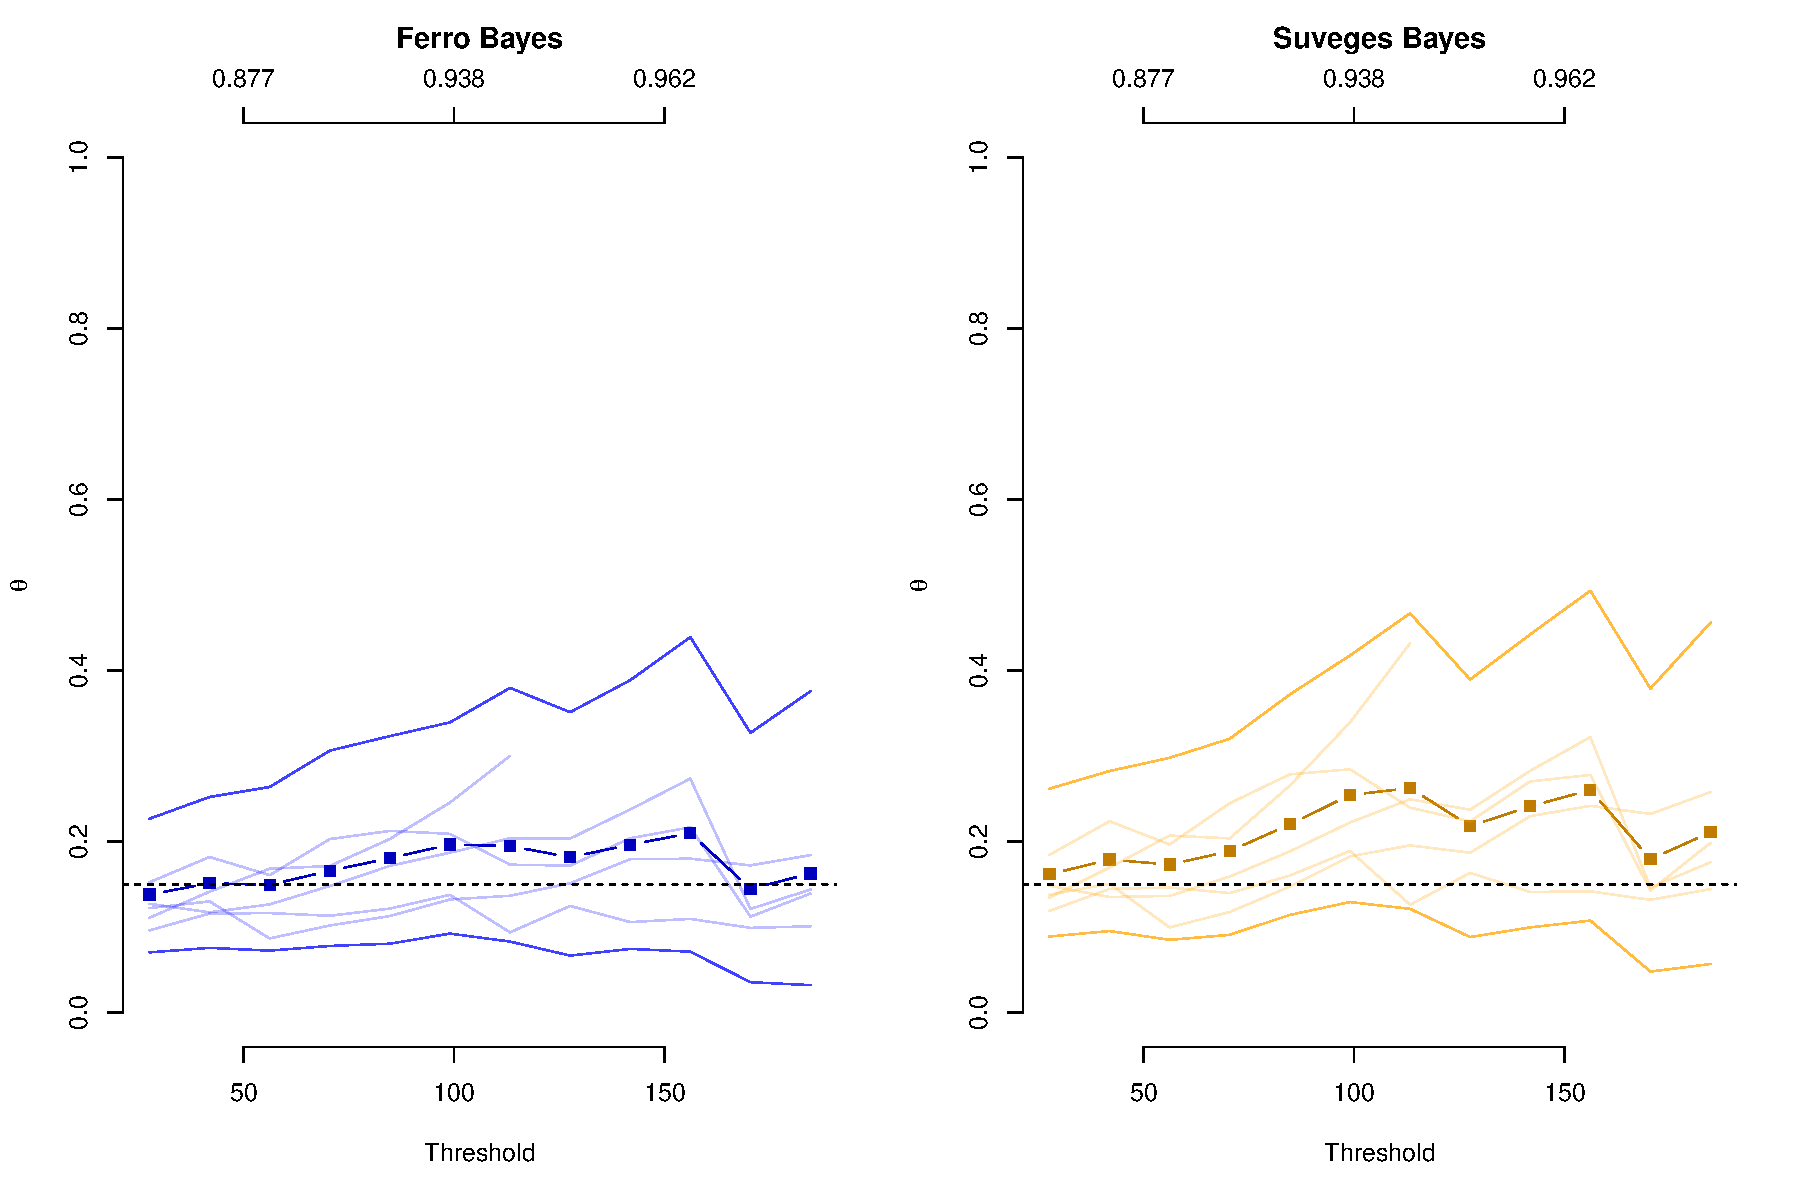
\includegraphics[width=5.5in, height=2.45in]{../extremal_comparison/figs/sim_frechet_hier_15_250_5.pdf}
\caption{$\theta=0.15$, $n=250$, $R=5$}
\end{center}
\end{figure}

\begin{figure}
\begin{center}
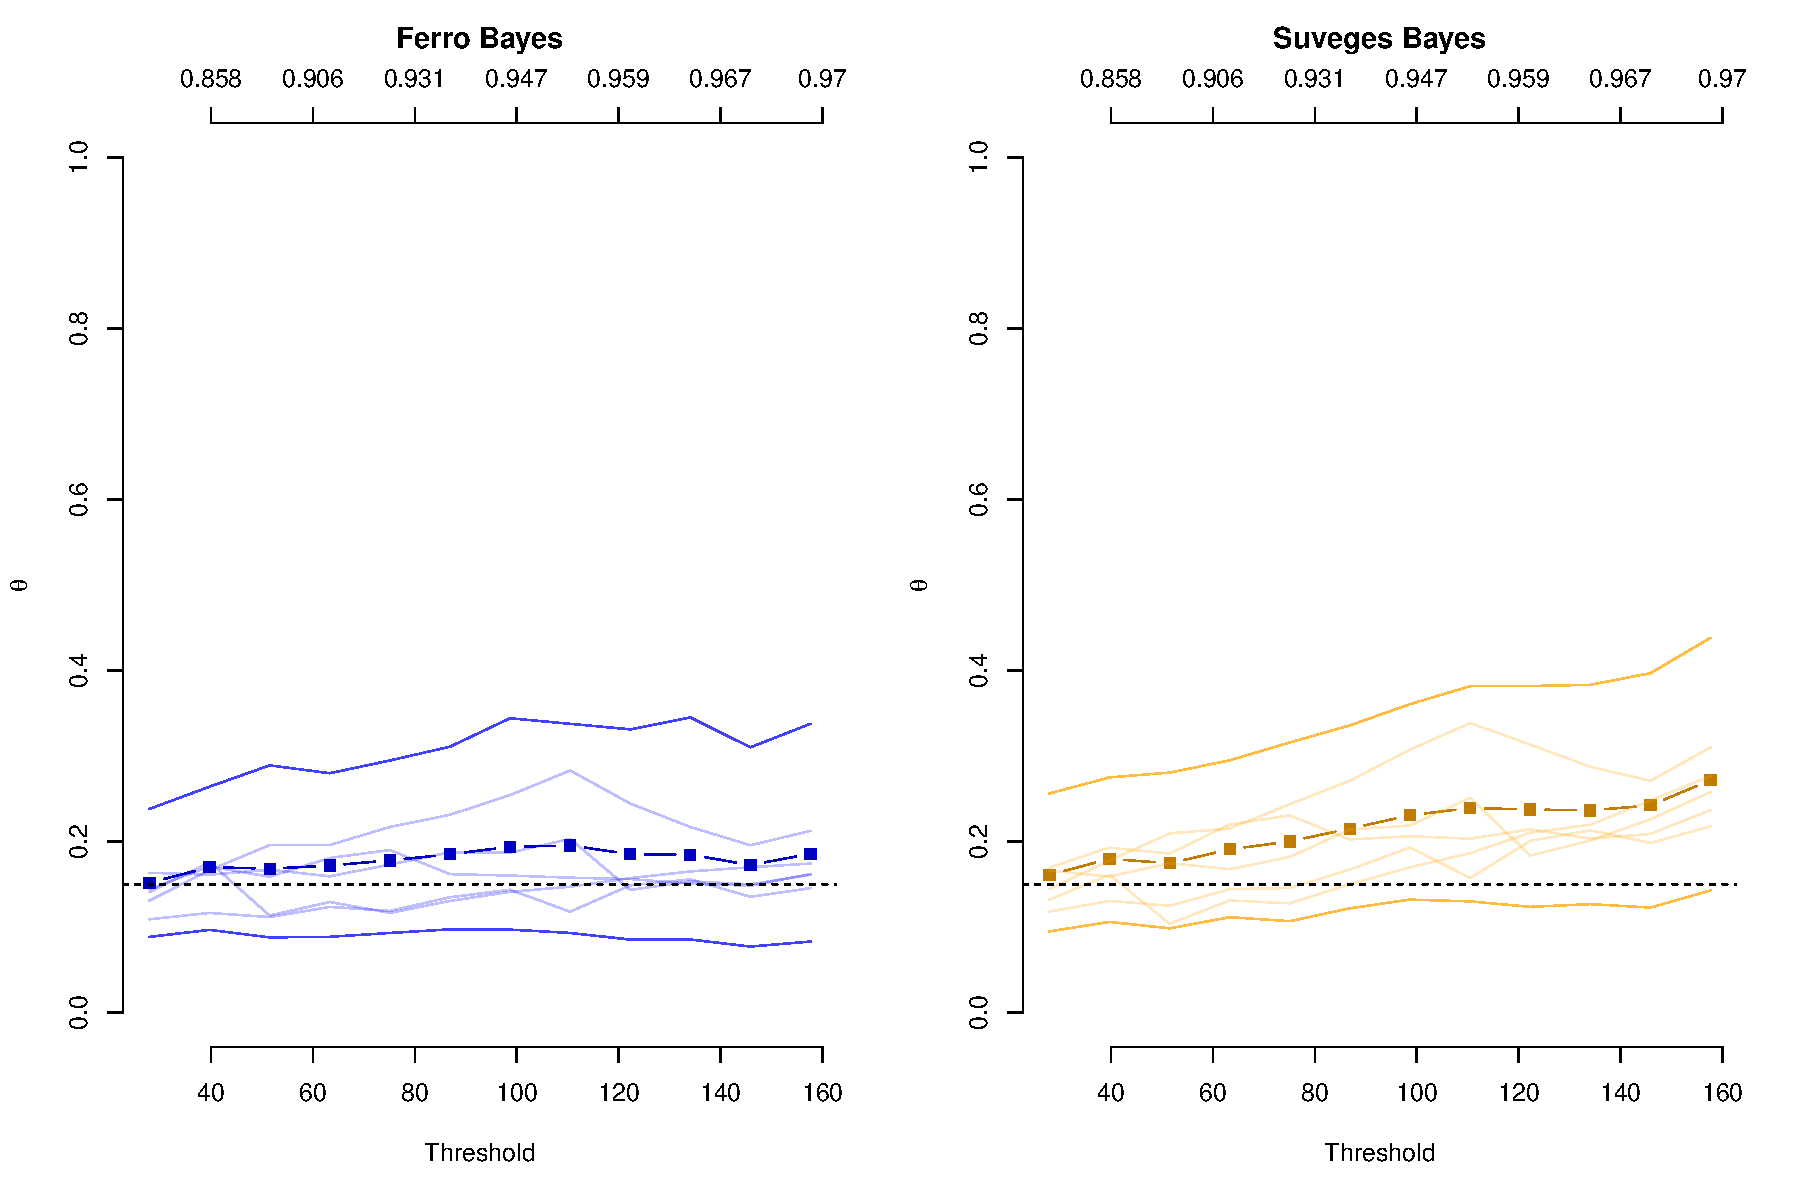
\includegraphics[width=5.5in, height=2.45in]{../extremal_comparison/figs/sim_frechet_hier_15_500_5.pdf}
\caption{$\theta=0.15$, $n=500$, $R=5$}
\end{center}
\end{figure}

\begin{figure}
\begin{center}
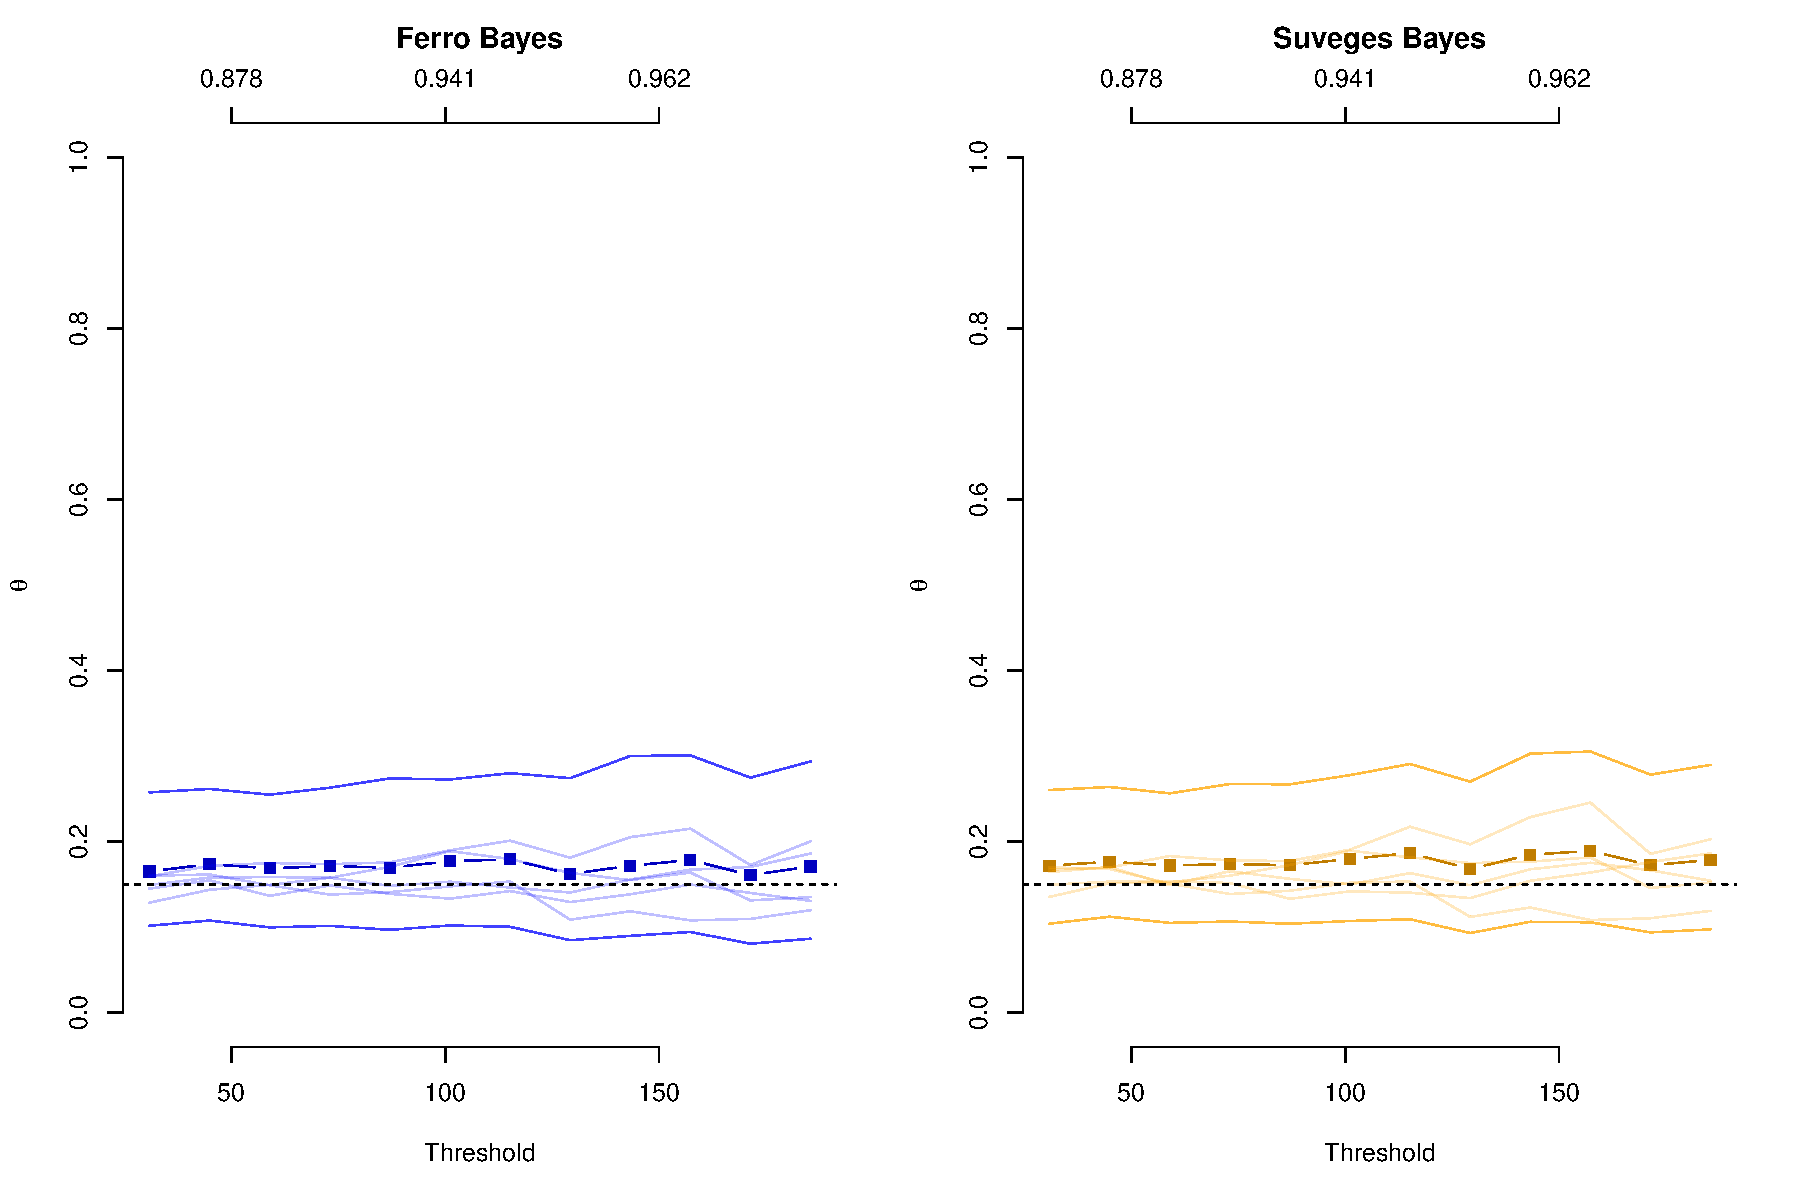
\includegraphics[width=5.5in, height=2.45in]{../extremal_comparison/figs/sim_frechet_hier_15_1000_5.pdf}
\caption{$\theta=0.15$, $n=1000$, $R=5$}
\end{center}
\end{figure}

\newpage

\begin{figure}
\begin{center}
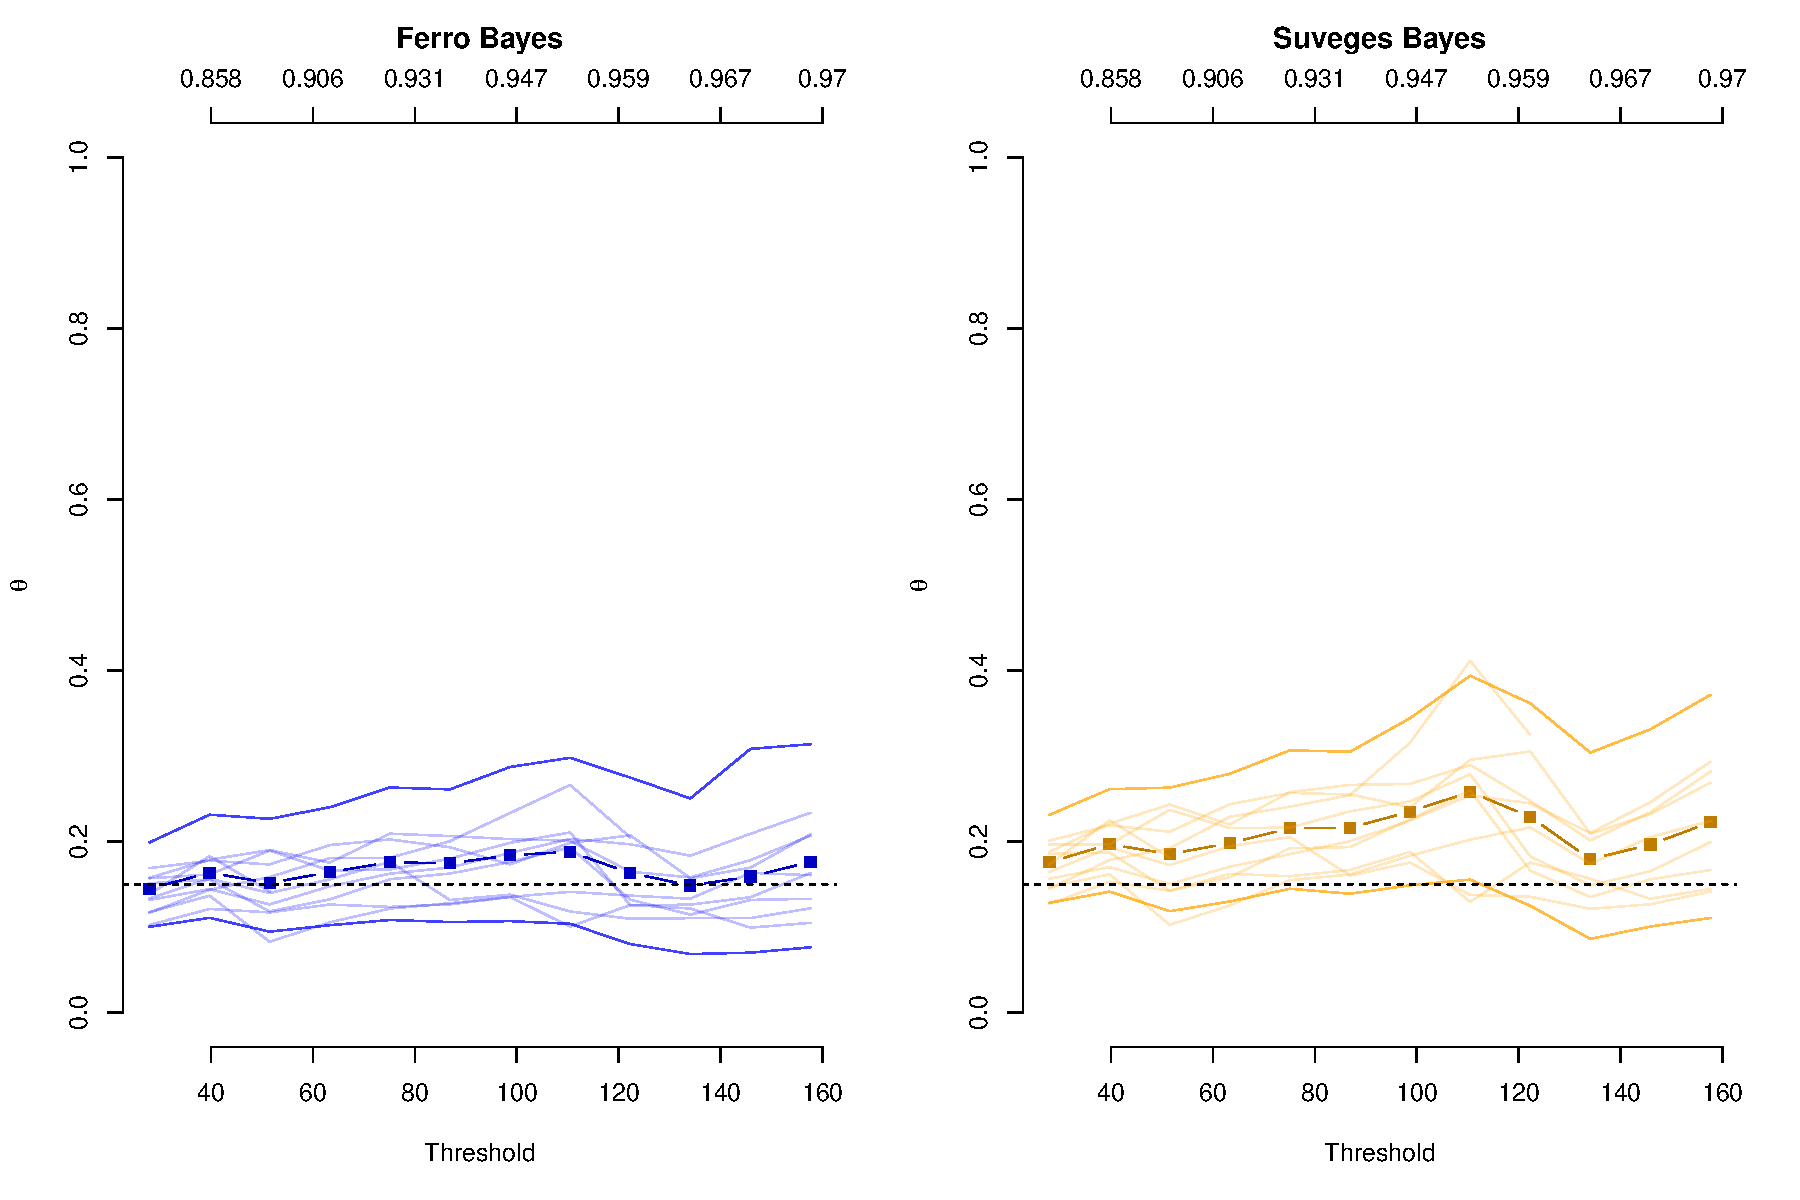
\includegraphics[width=5.5in, height=2.45in]{../extremal_comparison/figs/sim_frechet_hier_15_250_10.pdf}
\caption{$\theta=0.15$, $n=250$, $R=10$}
\end{center}
\end{figure}

\begin{figure}
\begin{center}
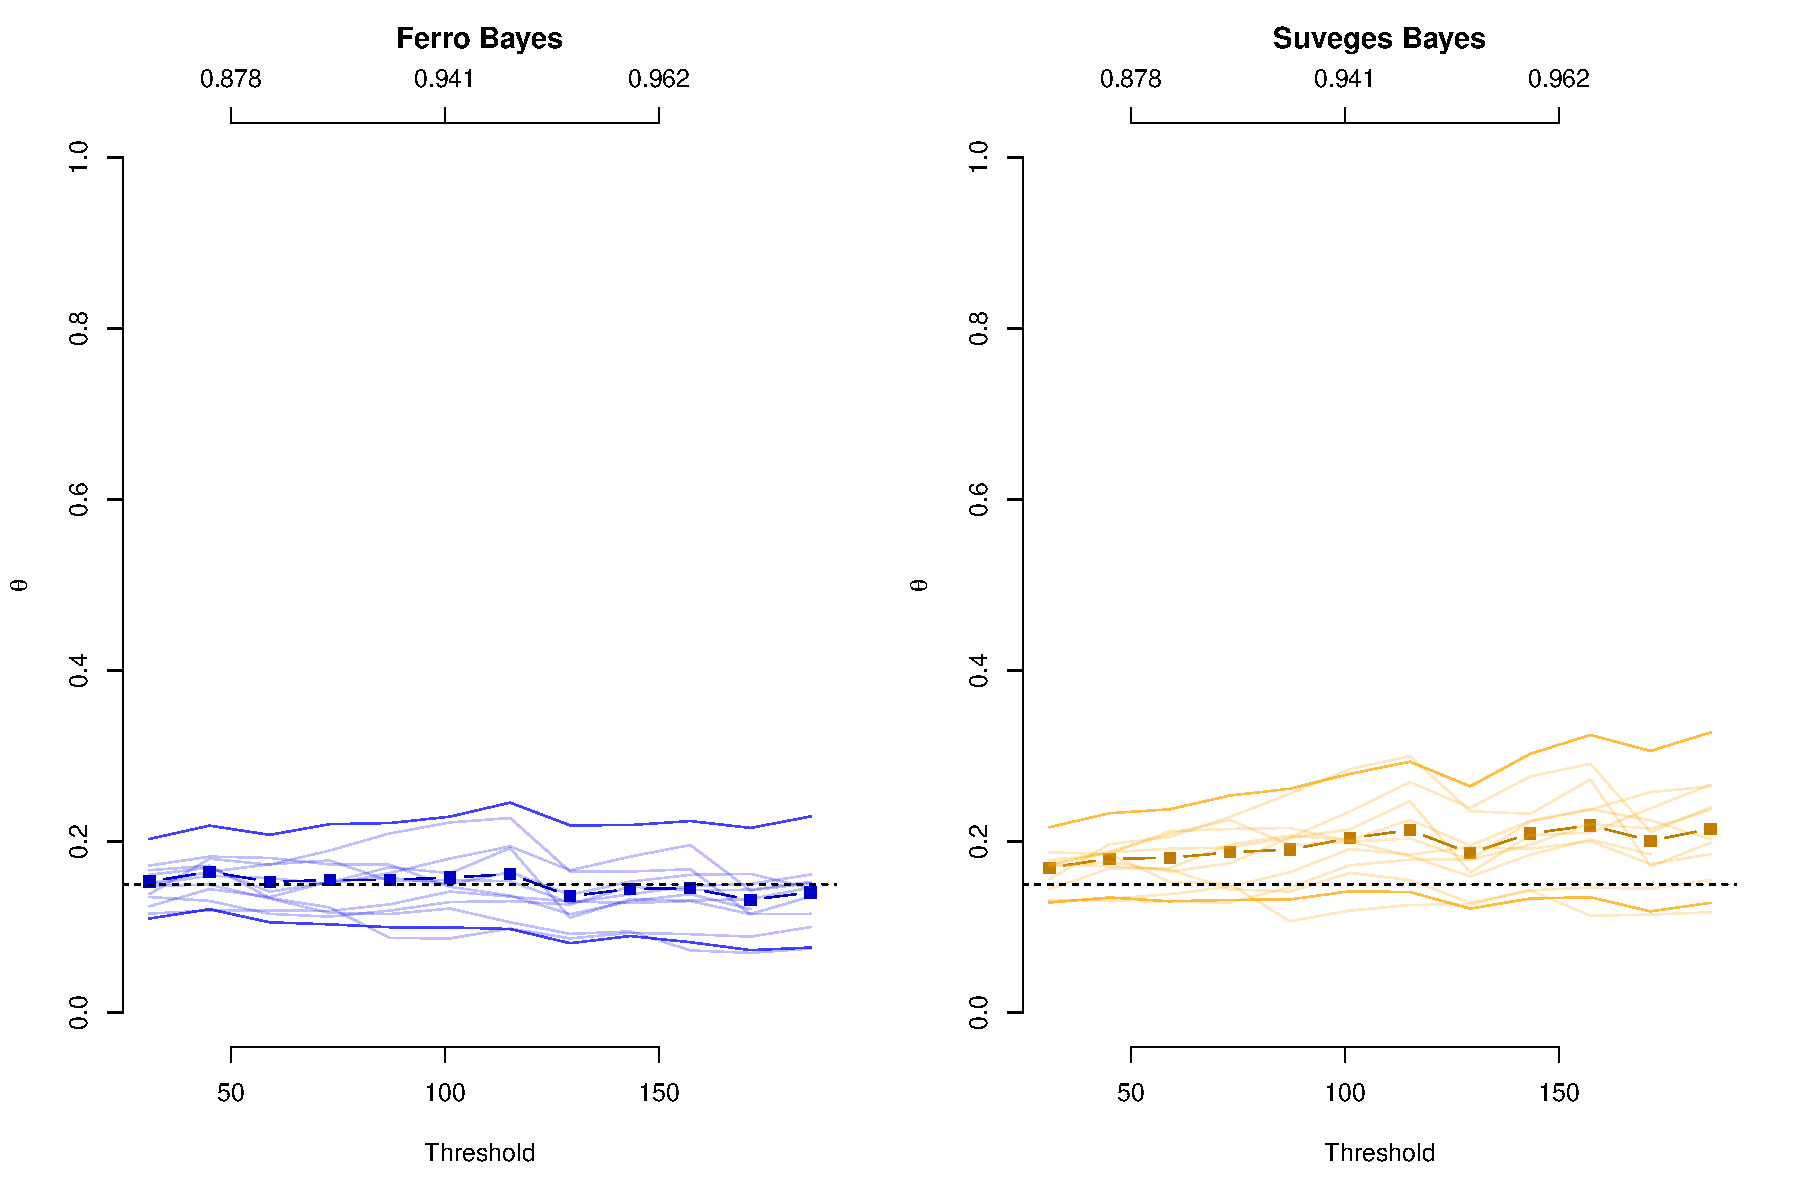
\includegraphics[width=5.5in, height=2.45in]{../extremal_comparison/figs/sim_frechet_hier_15_500_10.pdf}
\caption{$\theta=0.15$, $n=500$, $R=10$}
\end{center}
\end{figure}

\begin{figure}
\begin{center}
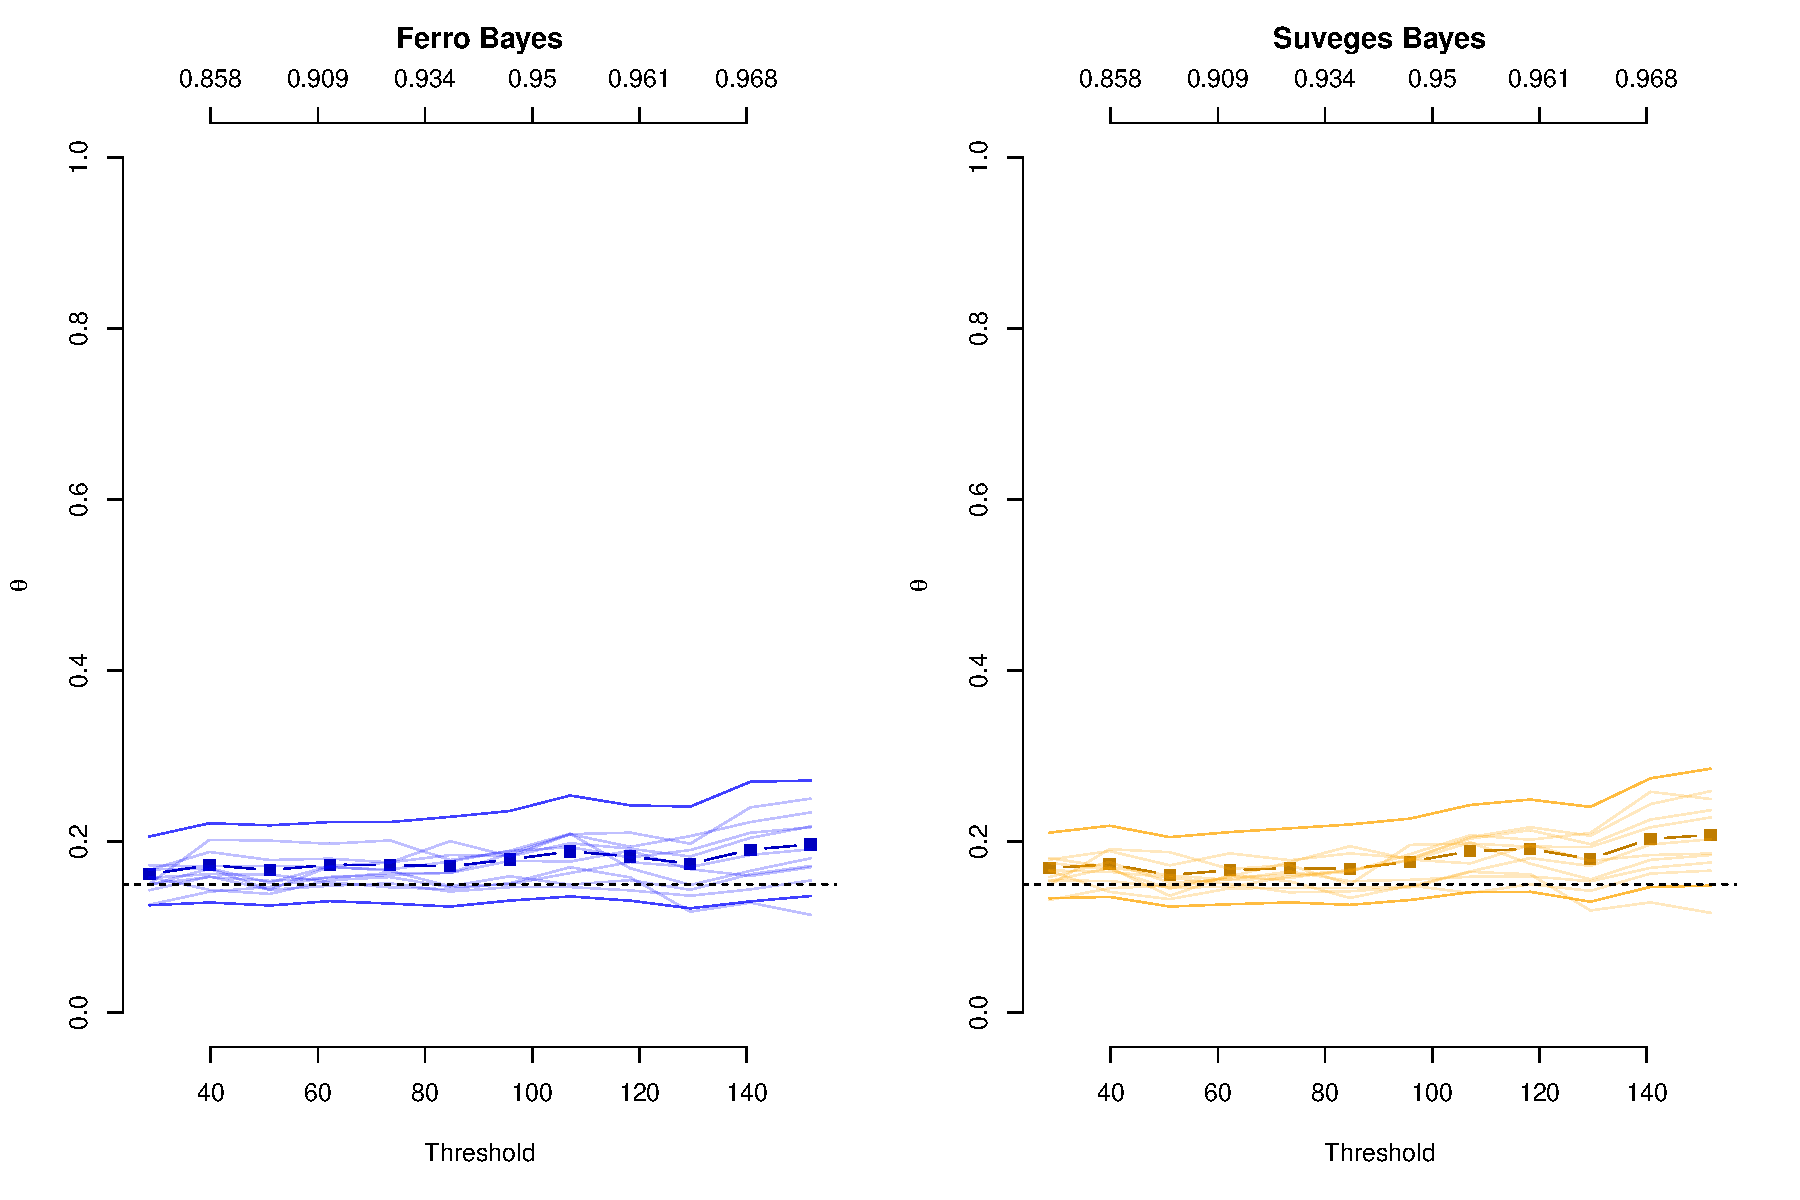
\includegraphics[width=5.5in, height=2.45in]{../extremal_comparison/figs/sim_frechet_hier_15_1000_10.pdf}
\caption{$\theta=0.15$, $n=1000$, $R=10$}
\end{center}
\end{figure}

\newpage

\begin{figure}
\begin{center}
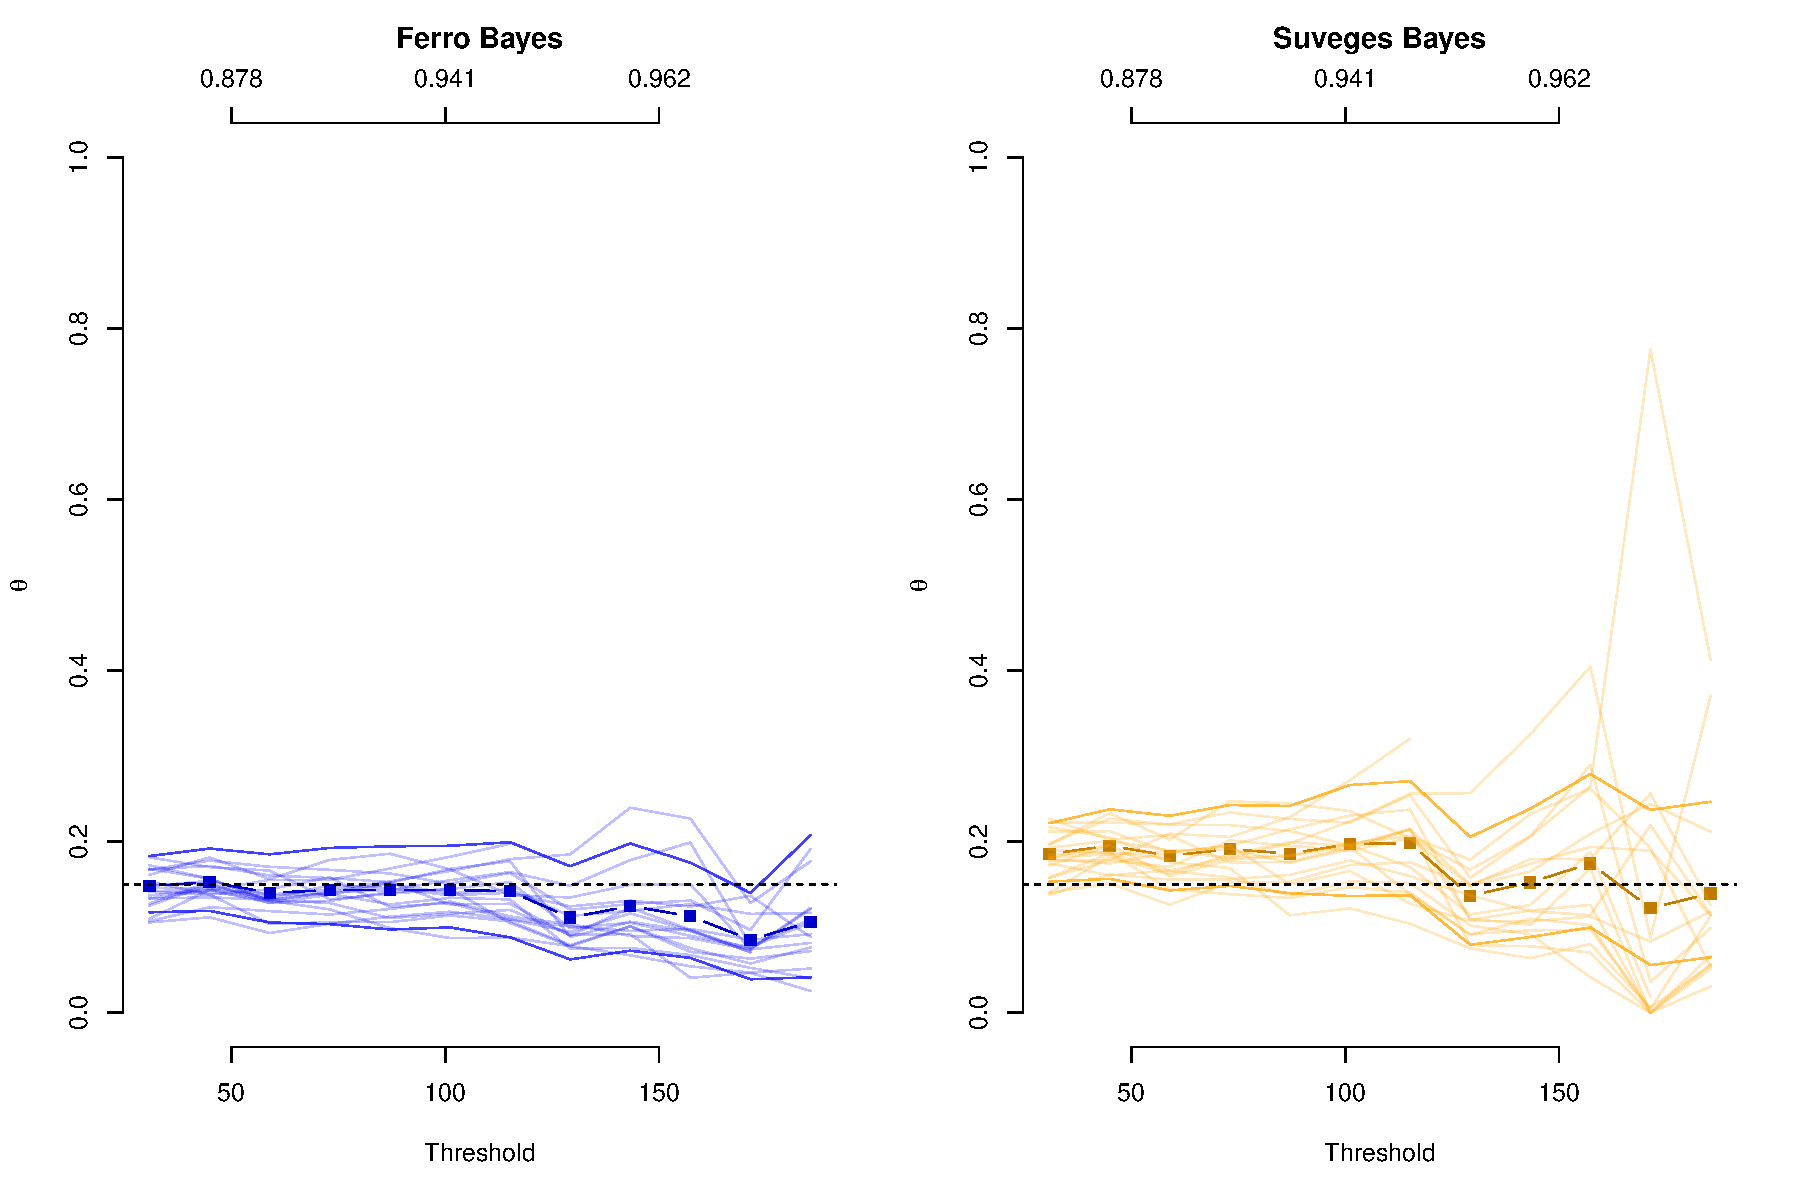
\includegraphics[width=5.5in, height=2.45in]{../extremal_comparison/figs/sim_frechet_hier_15_250_20.pdf}
\caption{$\theta=0.15$, $n=250$, $R=20$}
\end{center}
\end{figure}

\begin{figure}
\begin{center}
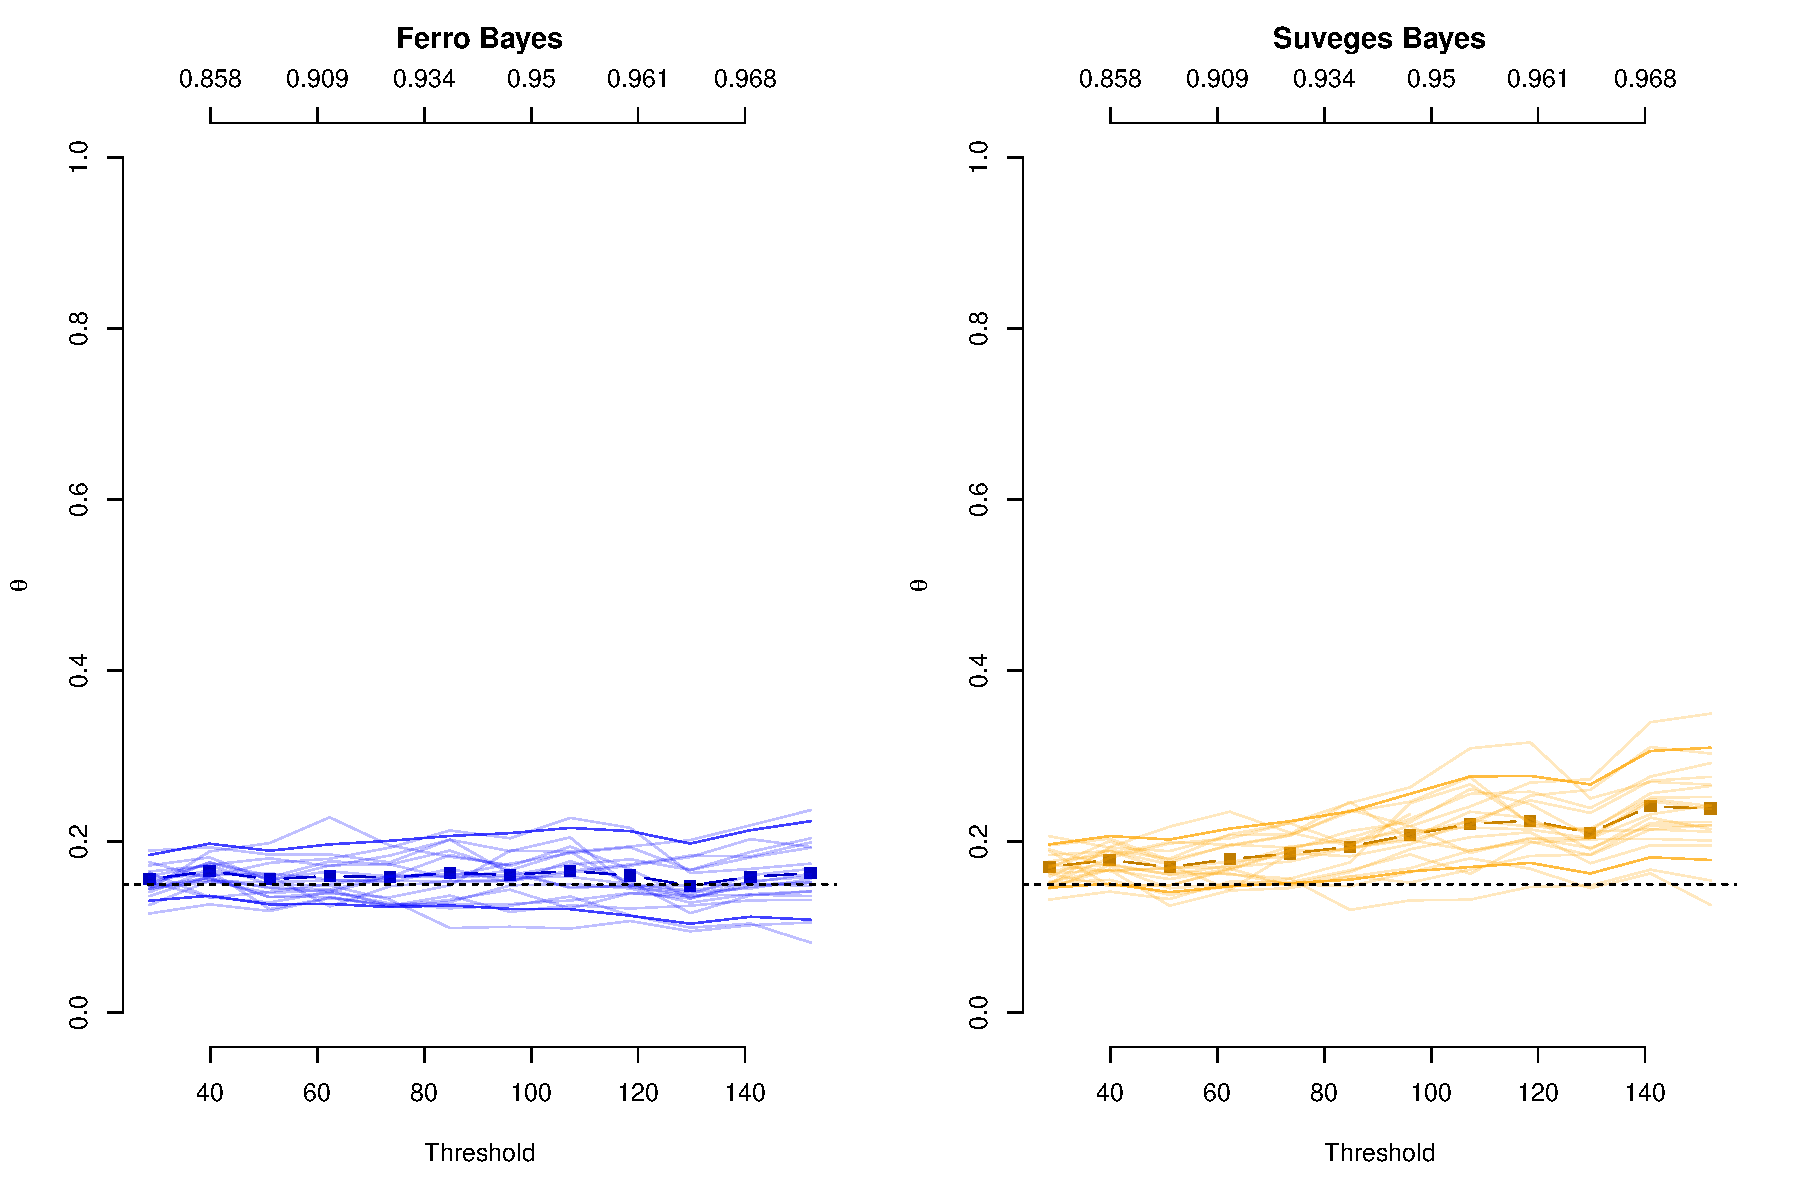
\includegraphics[width=5.5in, height=2.45in]{../extremal_comparison/figs/sim_frechet_hier_15_500_20.pdf}
\caption{$\theta=0.15$, $n=500$, $R=20$}
\end{center}
\end{figure}

\begin{figure}
\begin{center}
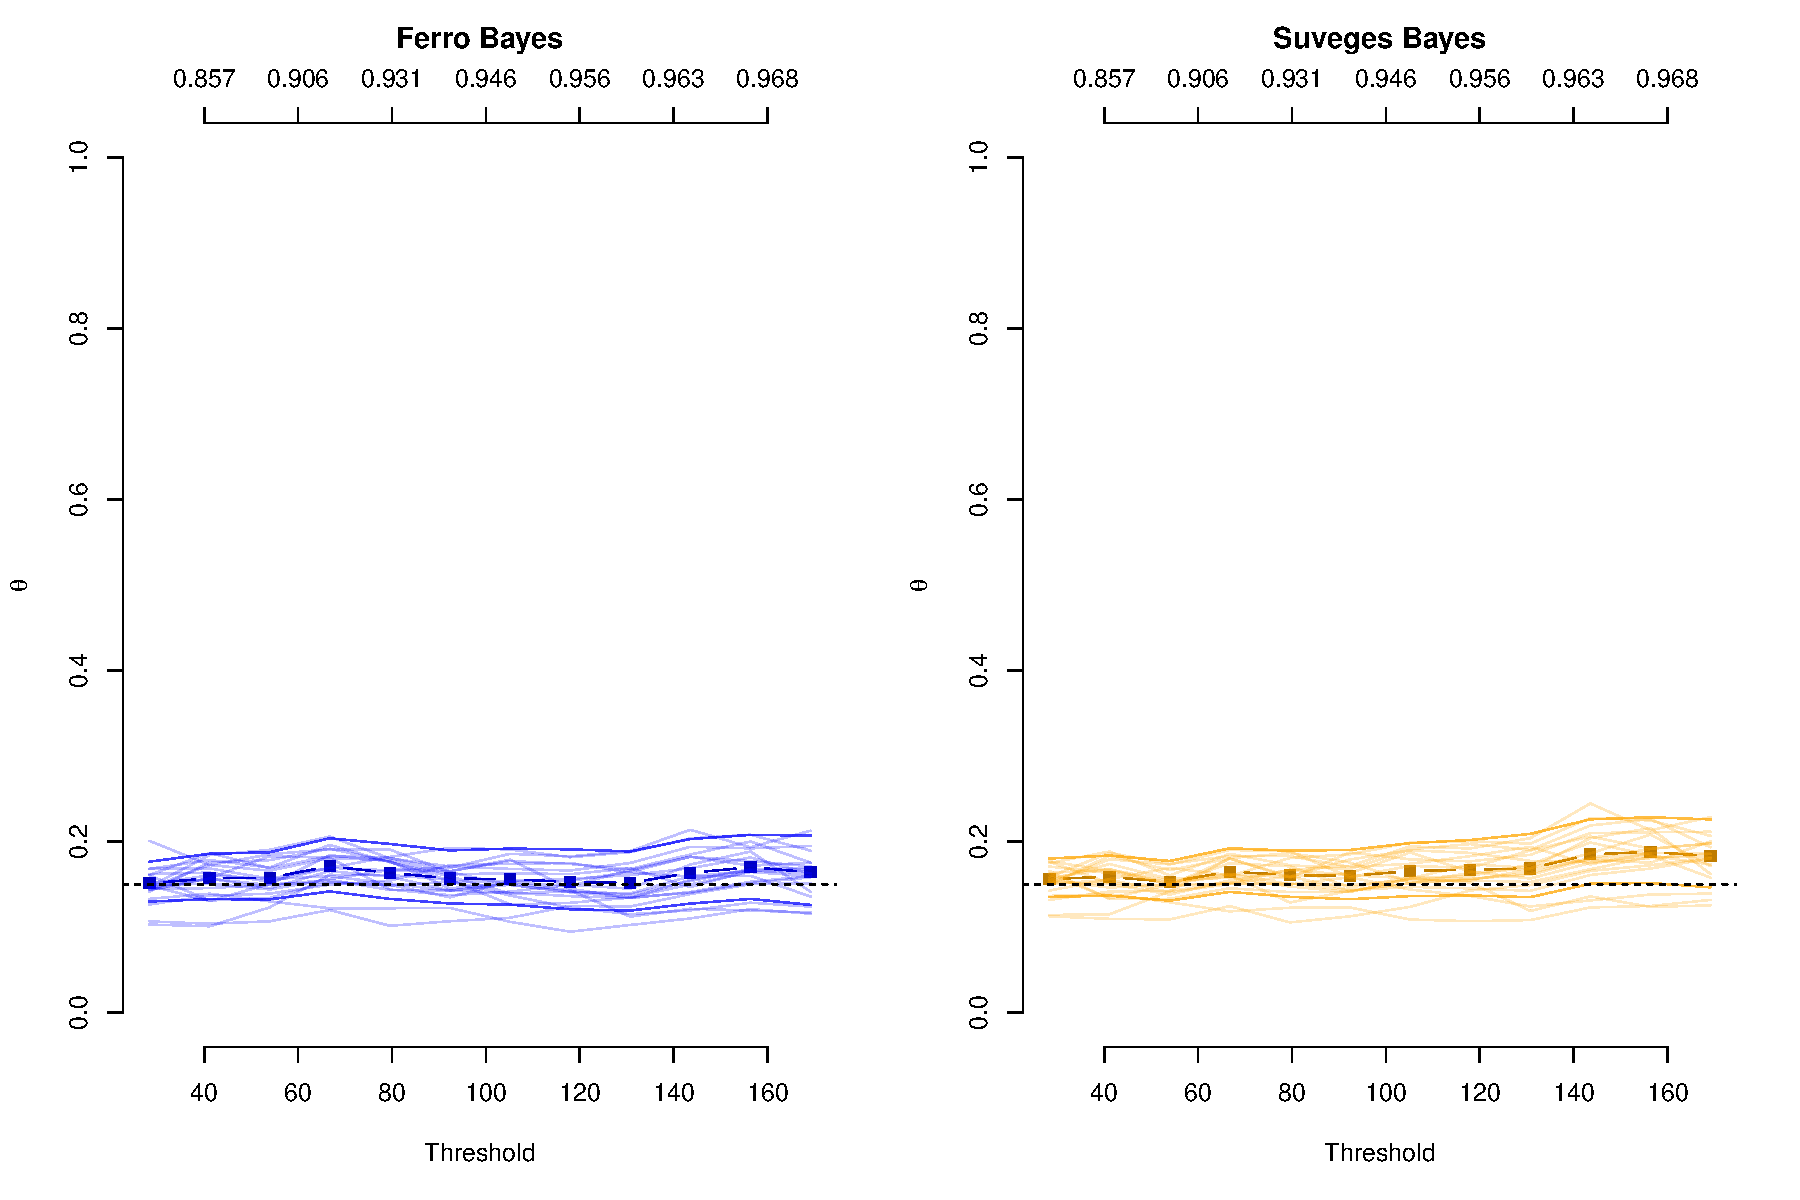
\includegraphics[width=5.5in, height=2.45in]{../extremal_comparison/figs/sim_frechet_hier_15_1000_20.pdf}
\caption{$\theta=0.15$, $n=1000$, $R=20$}
\end{center}
\end{figure}







\newpage

\begin{figure}
\begin{center}
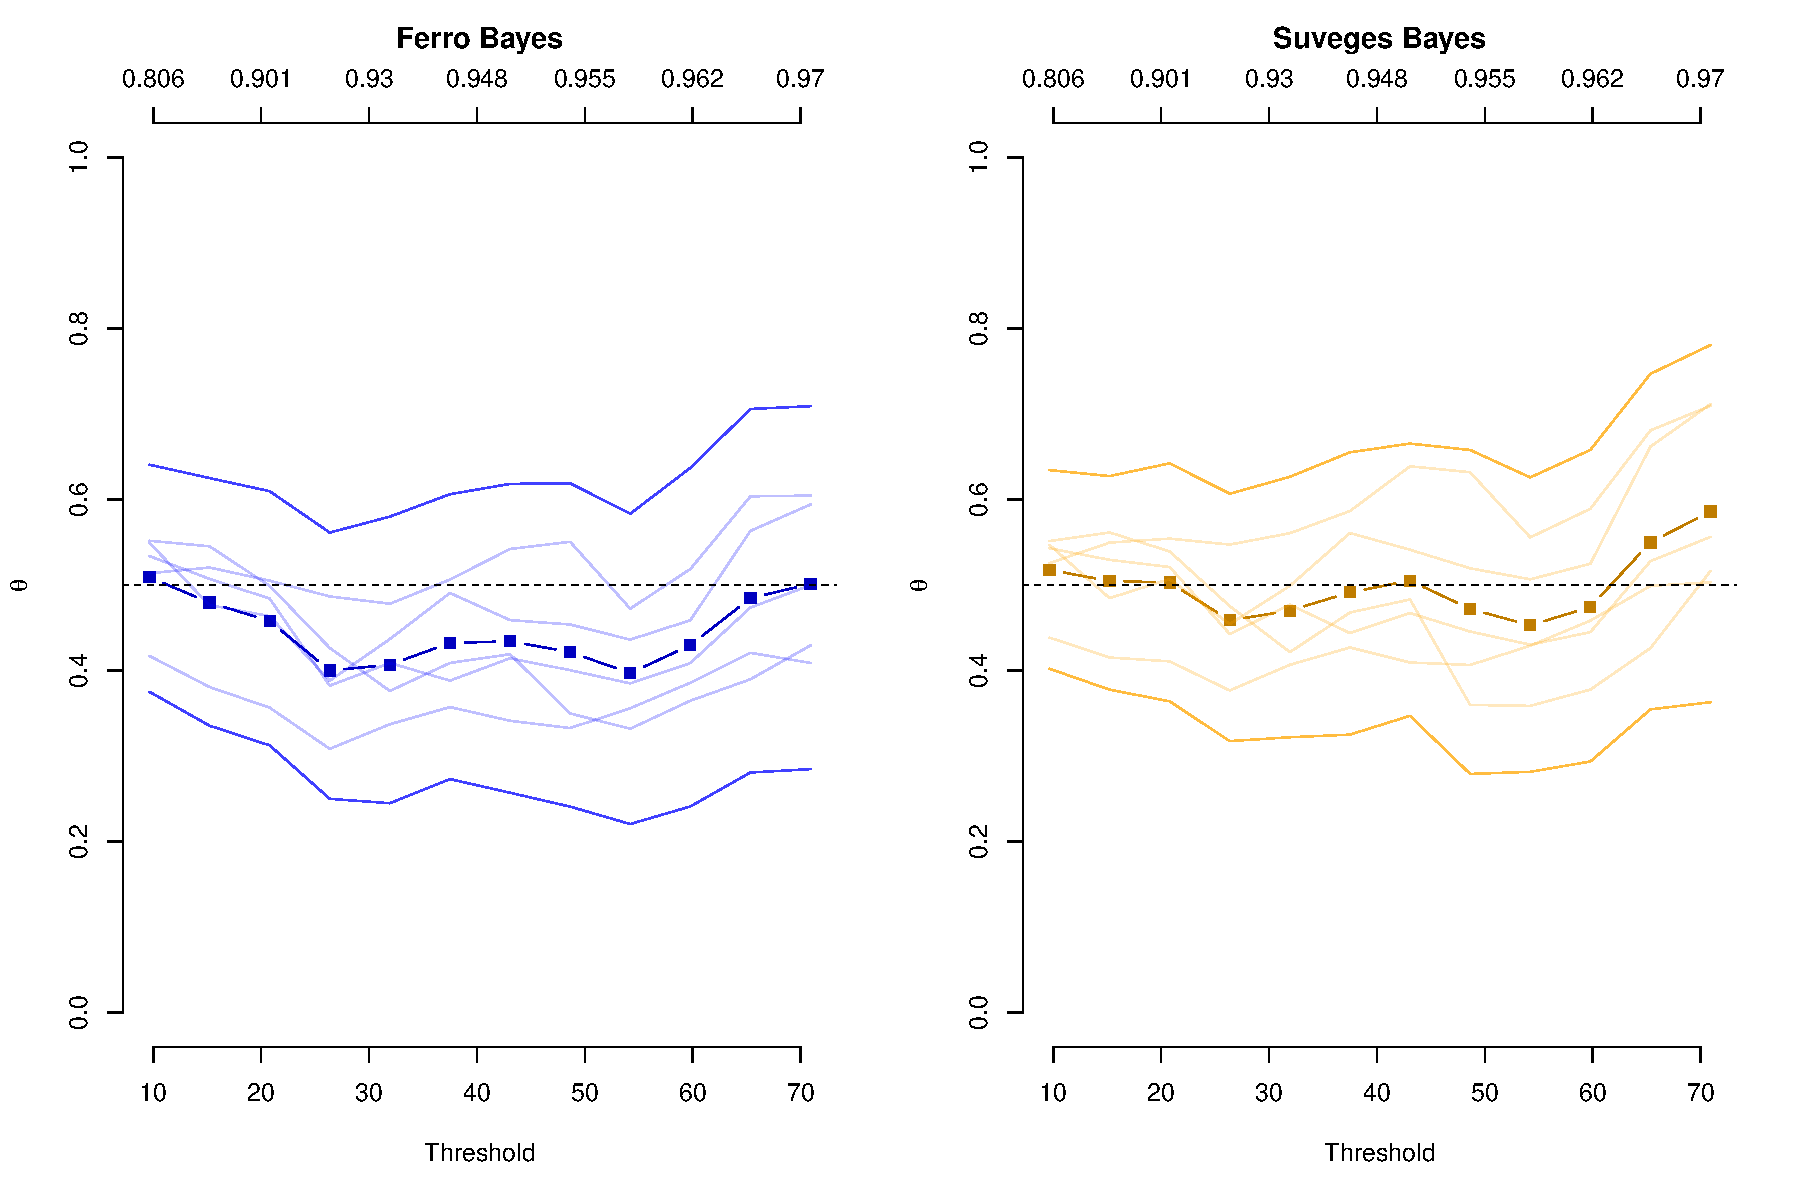
\includegraphics[width=5.5in, height=2.45in]{../extremal_comparison/figs/sim_frechet_hier_50_250_5.pdf}
\caption{$\theta=0.50$, $n=250$, $R=5$}
\end{center}
\end{figure}

\begin{figure}
\begin{center}
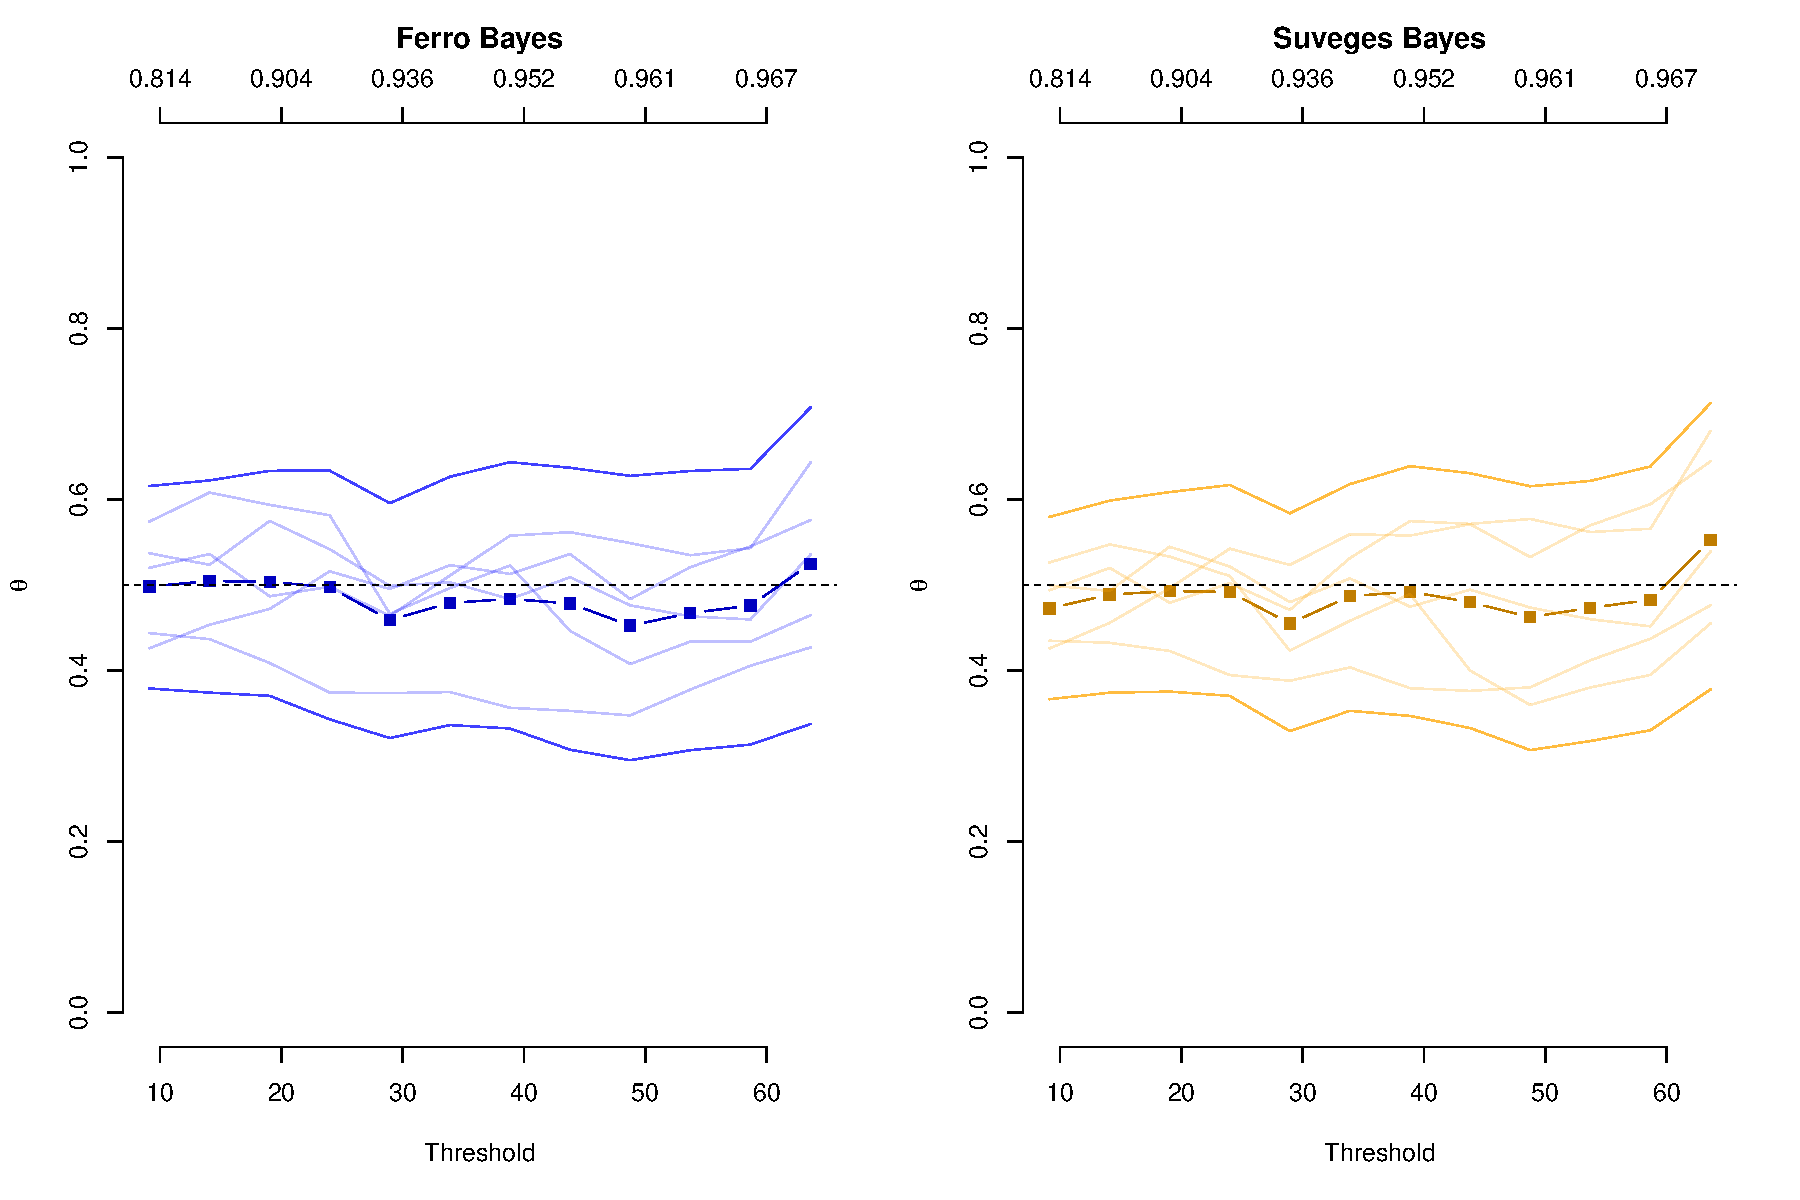
\includegraphics[width=5.5in, height=2.45in]{../extremal_comparison/figs/sim_frechet_hier_50_500_5.pdf}
\caption{$\theta=0.50$, $n=500$, $R=5$}
\end{center}
\end{figure}

\begin{figure}
\begin{center}
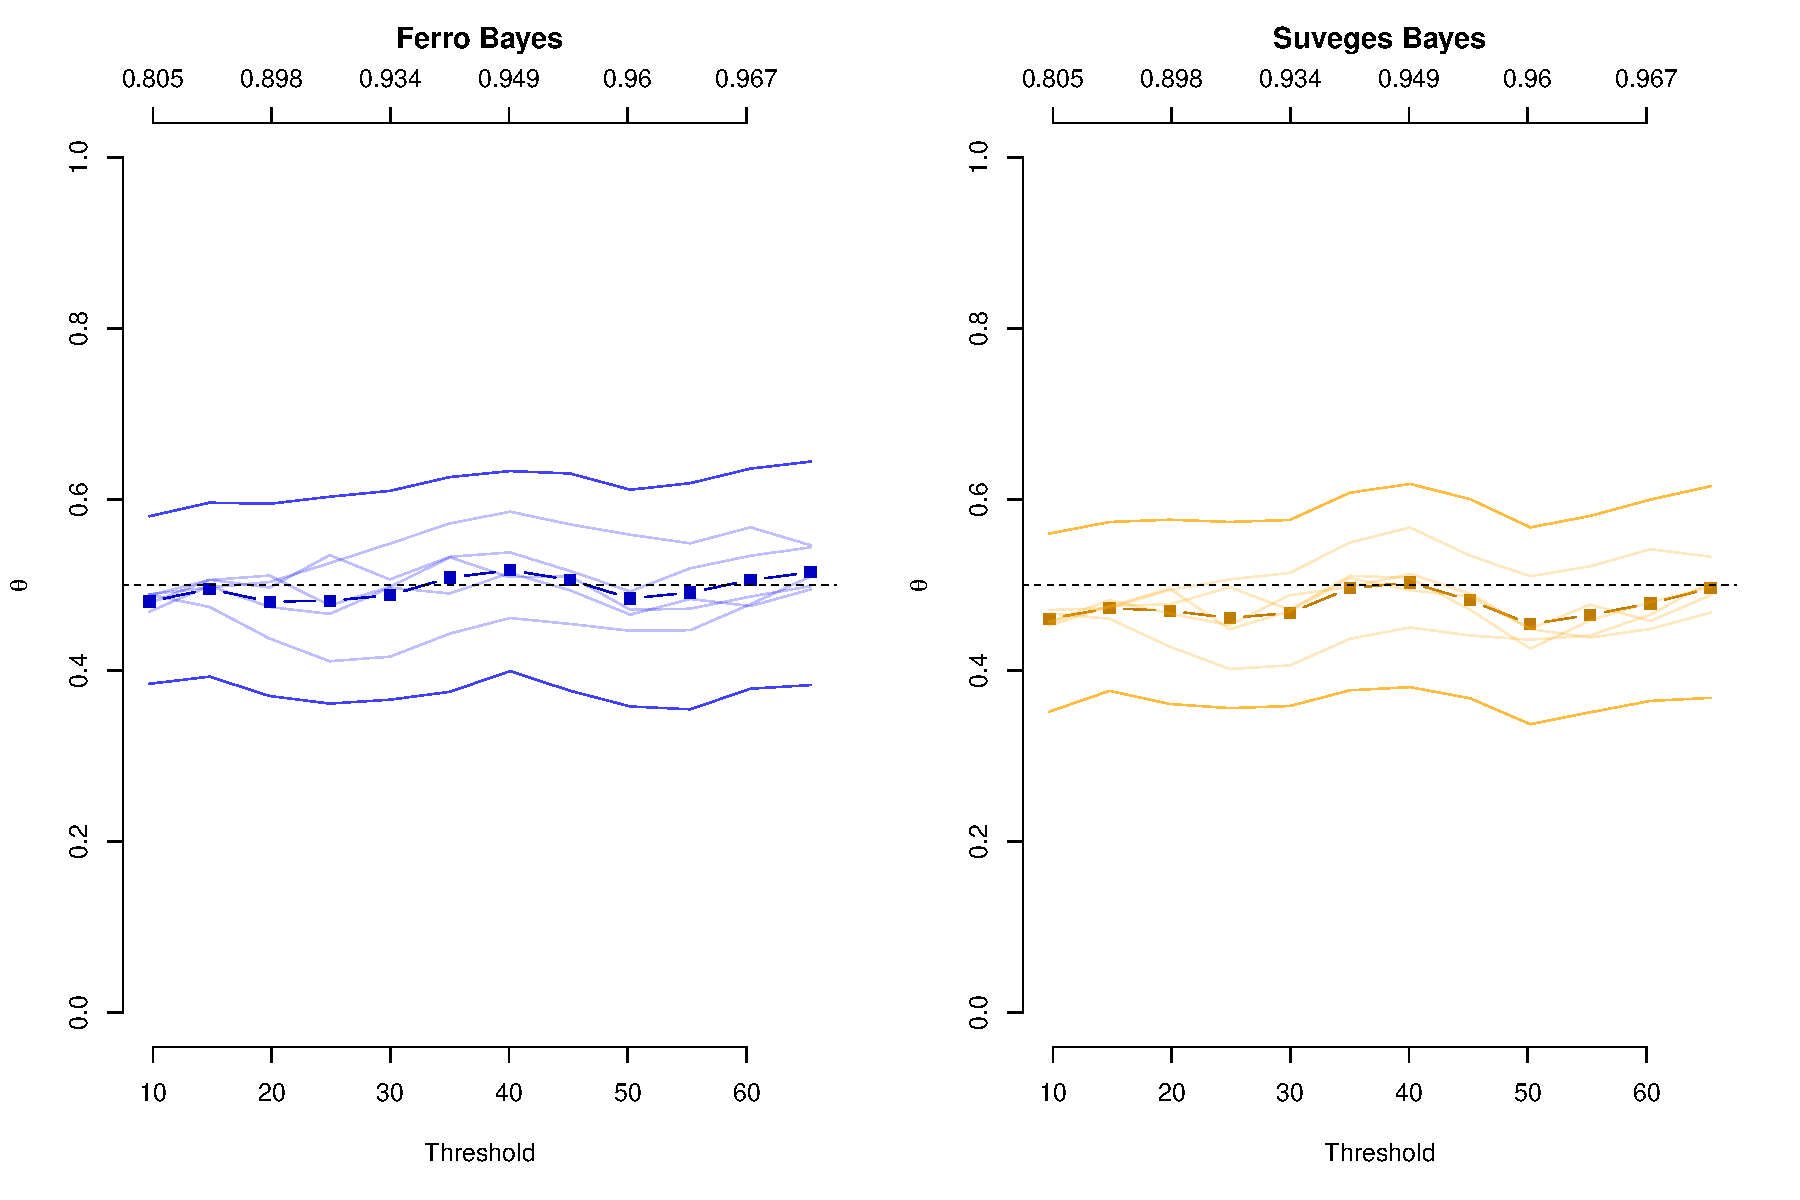
\includegraphics[width=5.5in, height=2.45in]{../extremal_comparison/figs/sim_frechet_hier_50_1000_5.pdf}
\caption{$\theta=0.50$, $n=1000$, $R=5$}
\end{center}
\end{figure}

\newpage

\begin{figure}
\begin{center}
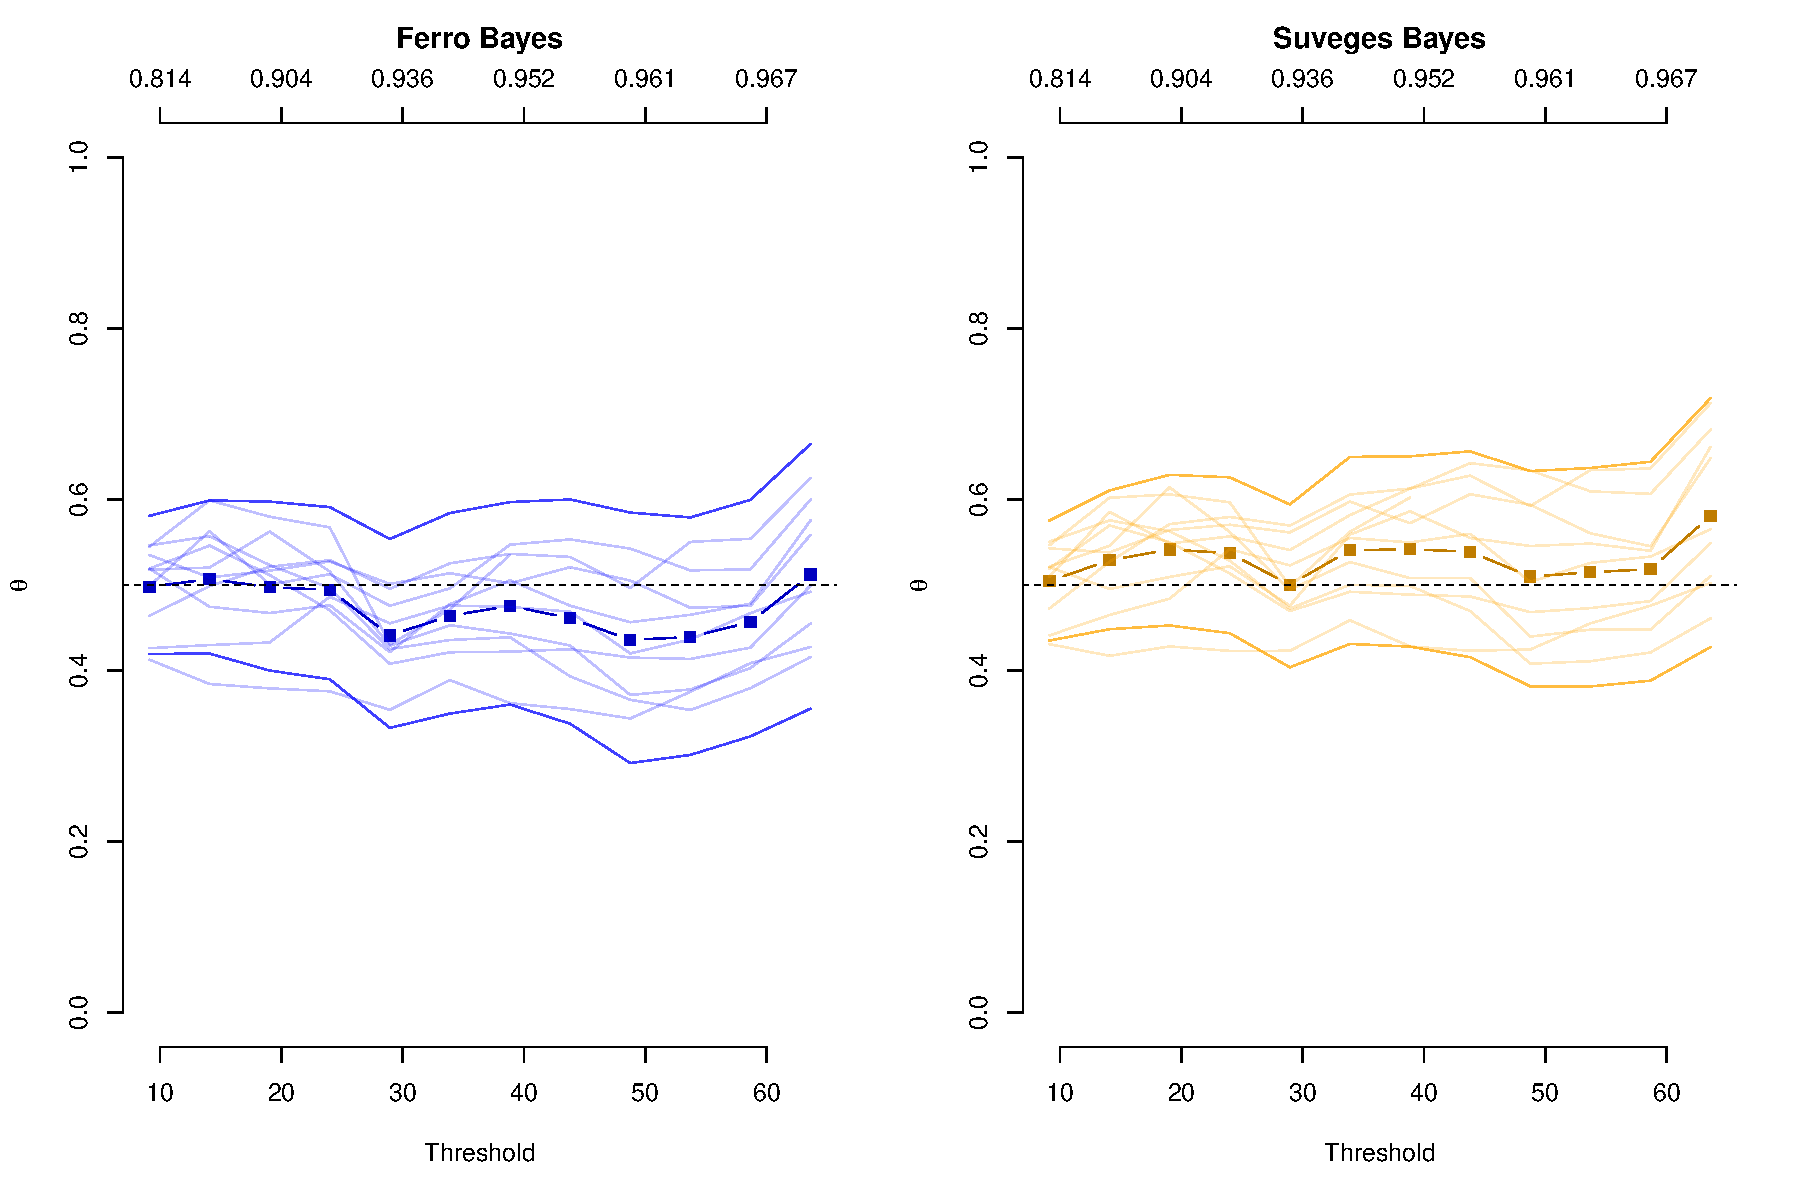
\includegraphics[width=5.5in, height=2.45in]{../extremal_comparison/figs/sim_frechet_hier_50_250_10.pdf}
\caption{$\theta=0.50$, $n=250$, $R=10$}
\end{center}
\end{figure}

\begin{figure}
\begin{center}
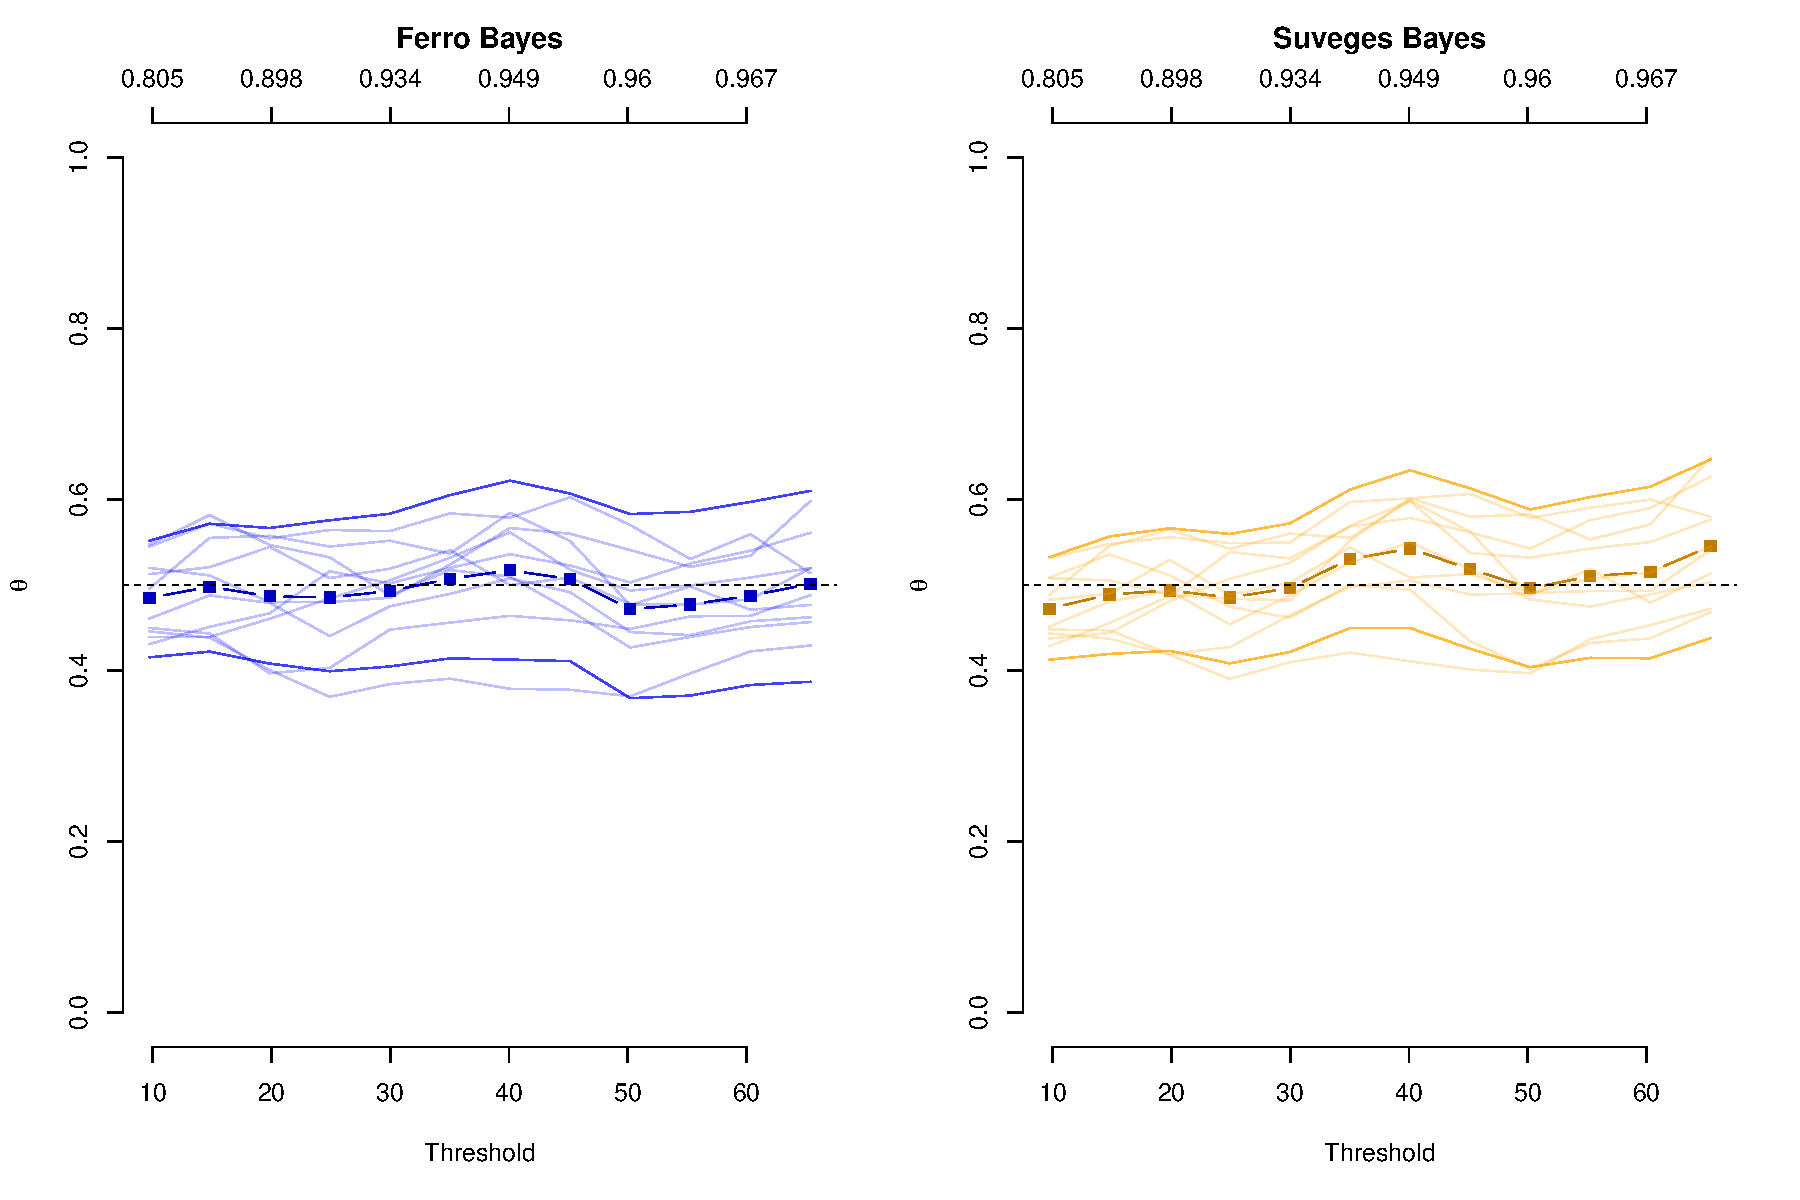
\includegraphics[width=5.5in, height=2.45in]{../extremal_comparison/figs/sim_frechet_hier_50_500_10.pdf}
\caption{$\theta=0.50$, $n=500$, $R=10$}
\end{center}
\end{figure}

\begin{figure}
\begin{center}
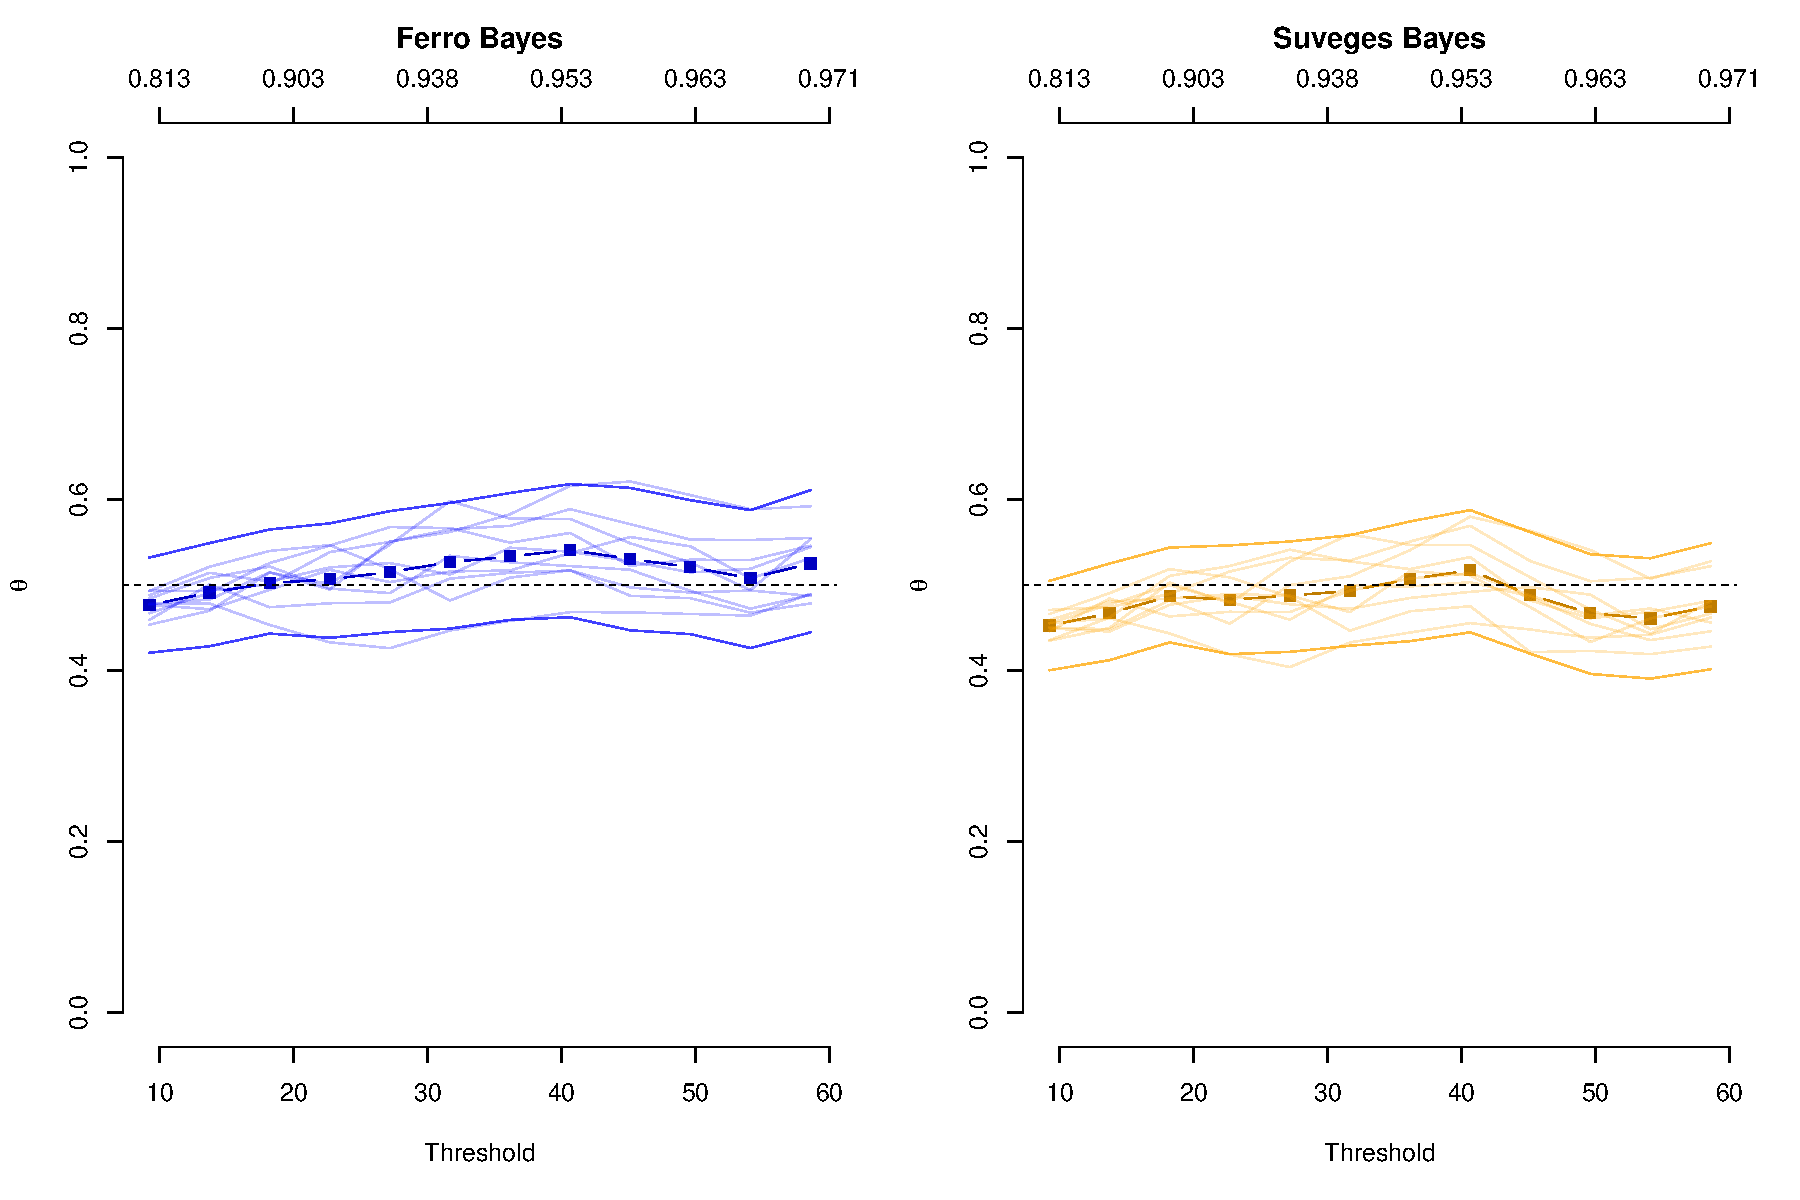
\includegraphics[width=5.5in, height=2.45in]{../extremal_comparison/figs/sim_frechet_hier_50_1000_10.pdf}
\caption{$\theta=0.50$, $n=1000$, $R=10$}
\end{center}
\end{figure}

\newpage

\begin{figure}
\begin{center}
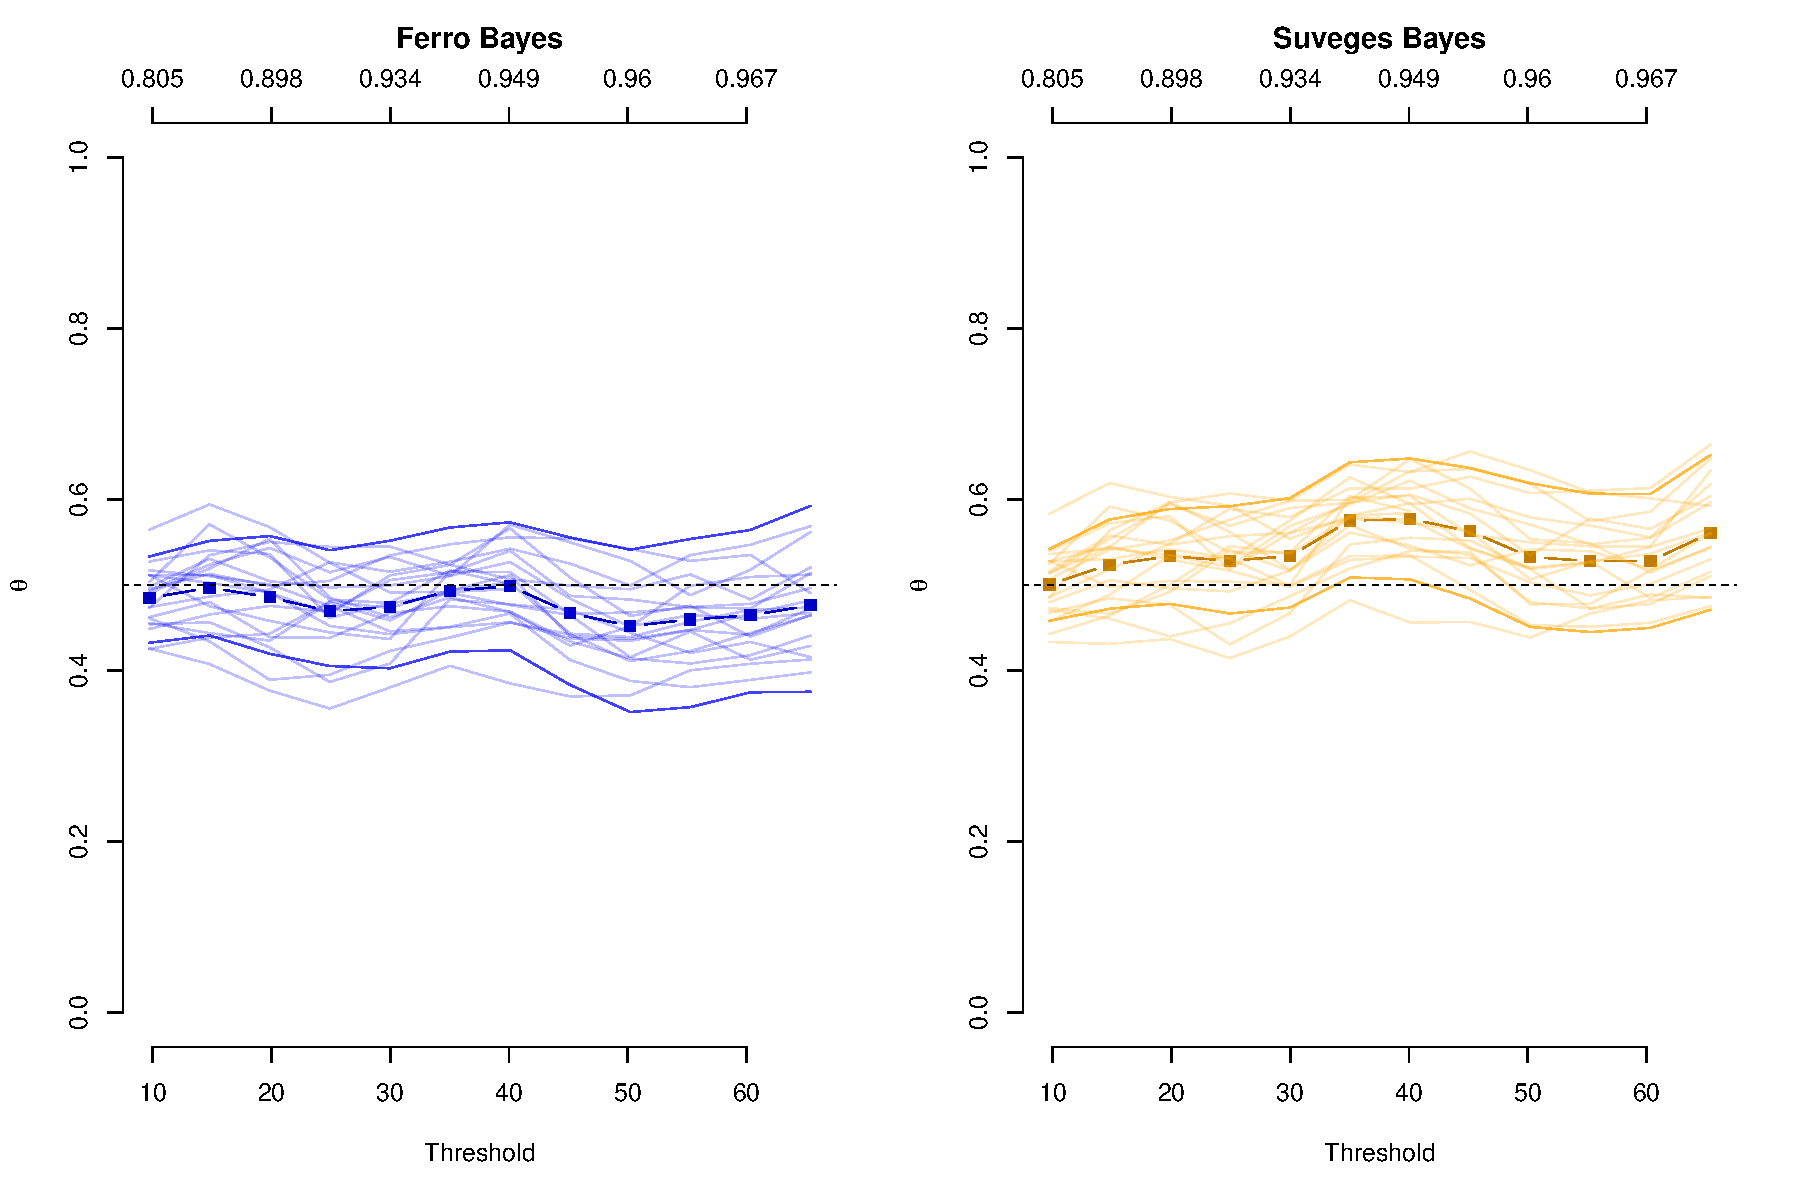
\includegraphics[width=5.5in, height=2.45in]{../extremal_comparison/figs/sim_frechet_hier_50_250_20.pdf}
\caption{$\theta=0.50$, $n=250$, $R=20$}
\end{center}
\end{figure}

\begin{figure}
\begin{center}
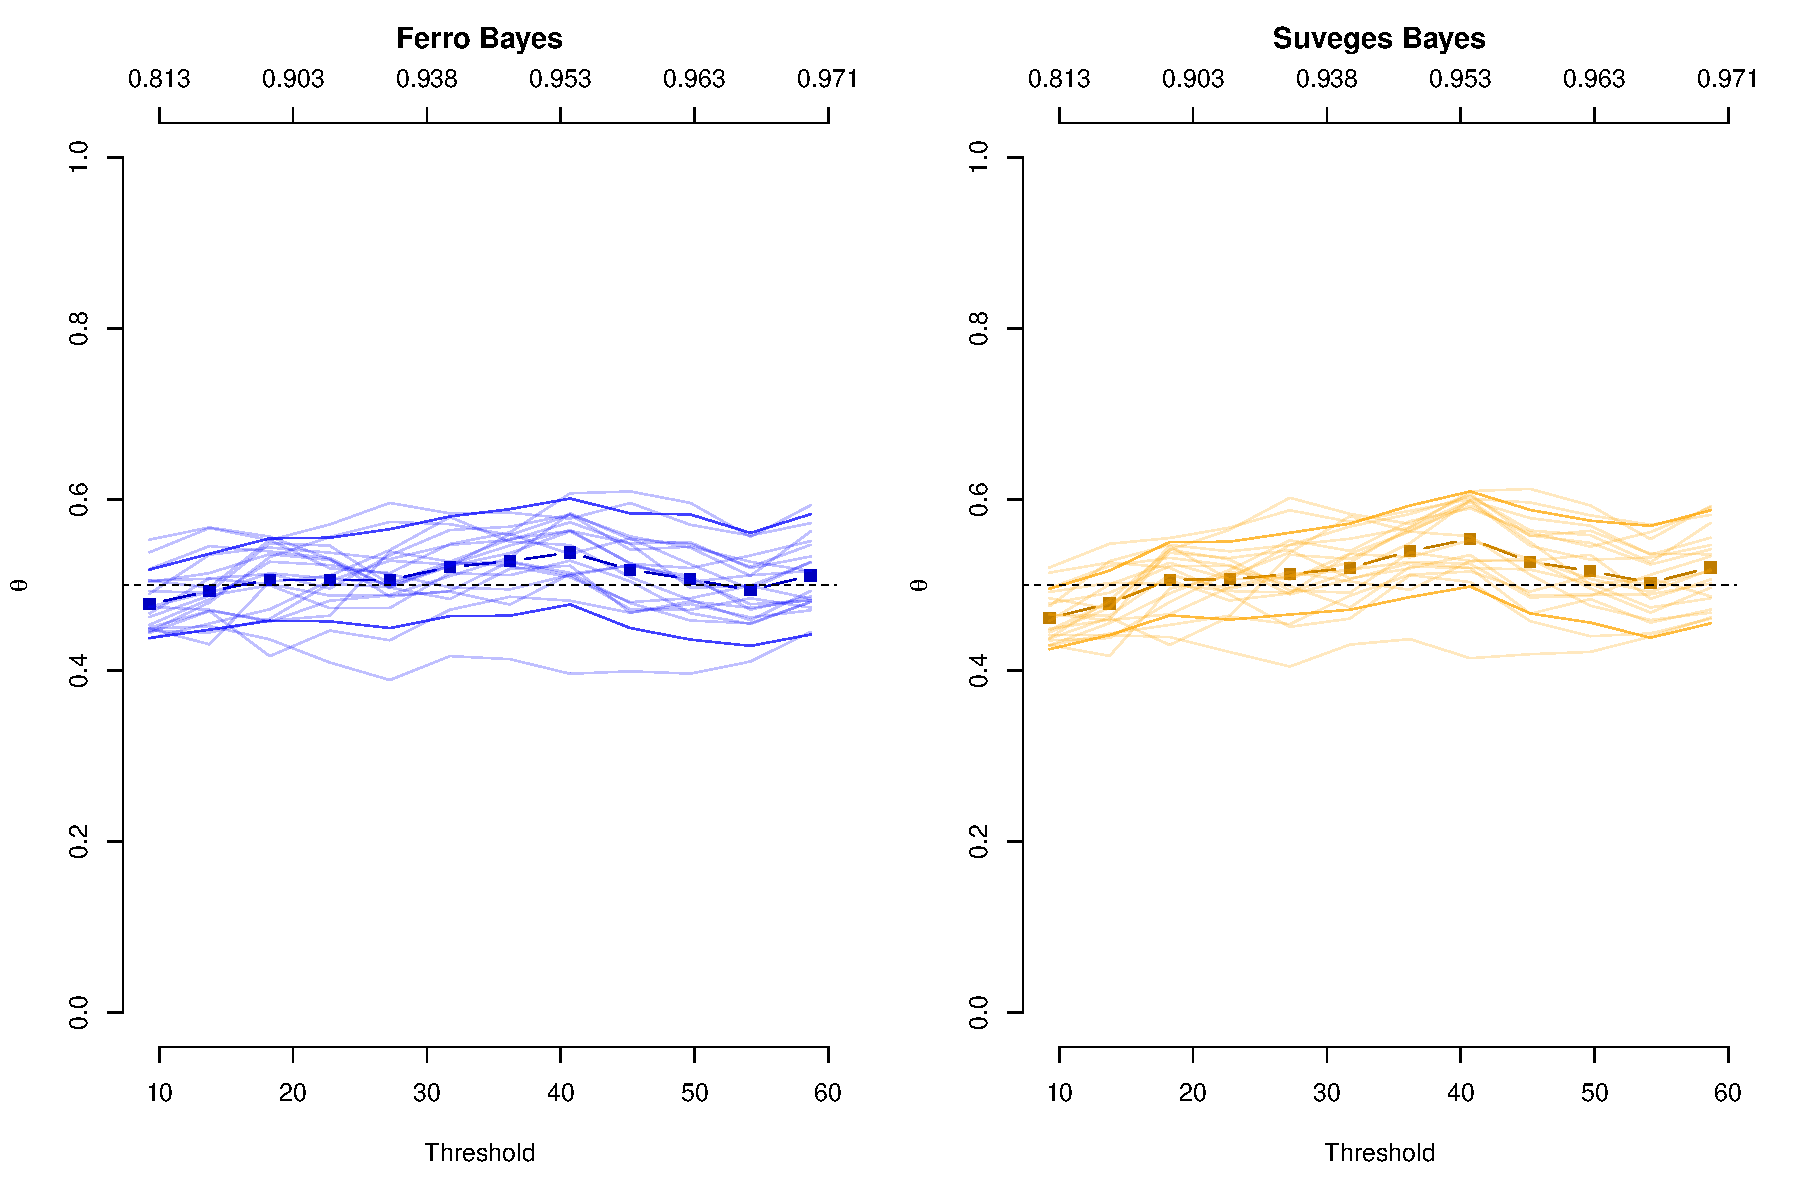
\includegraphics[width=5.5in, height=2.45in]{../extremal_comparison/figs/sim_frechet_hier_50_500_20.pdf}
\caption{$\theta=0.50$, $n=500$, $R=20$}
\end{center}
\end{figure}

\begin{figure}
\begin{center}
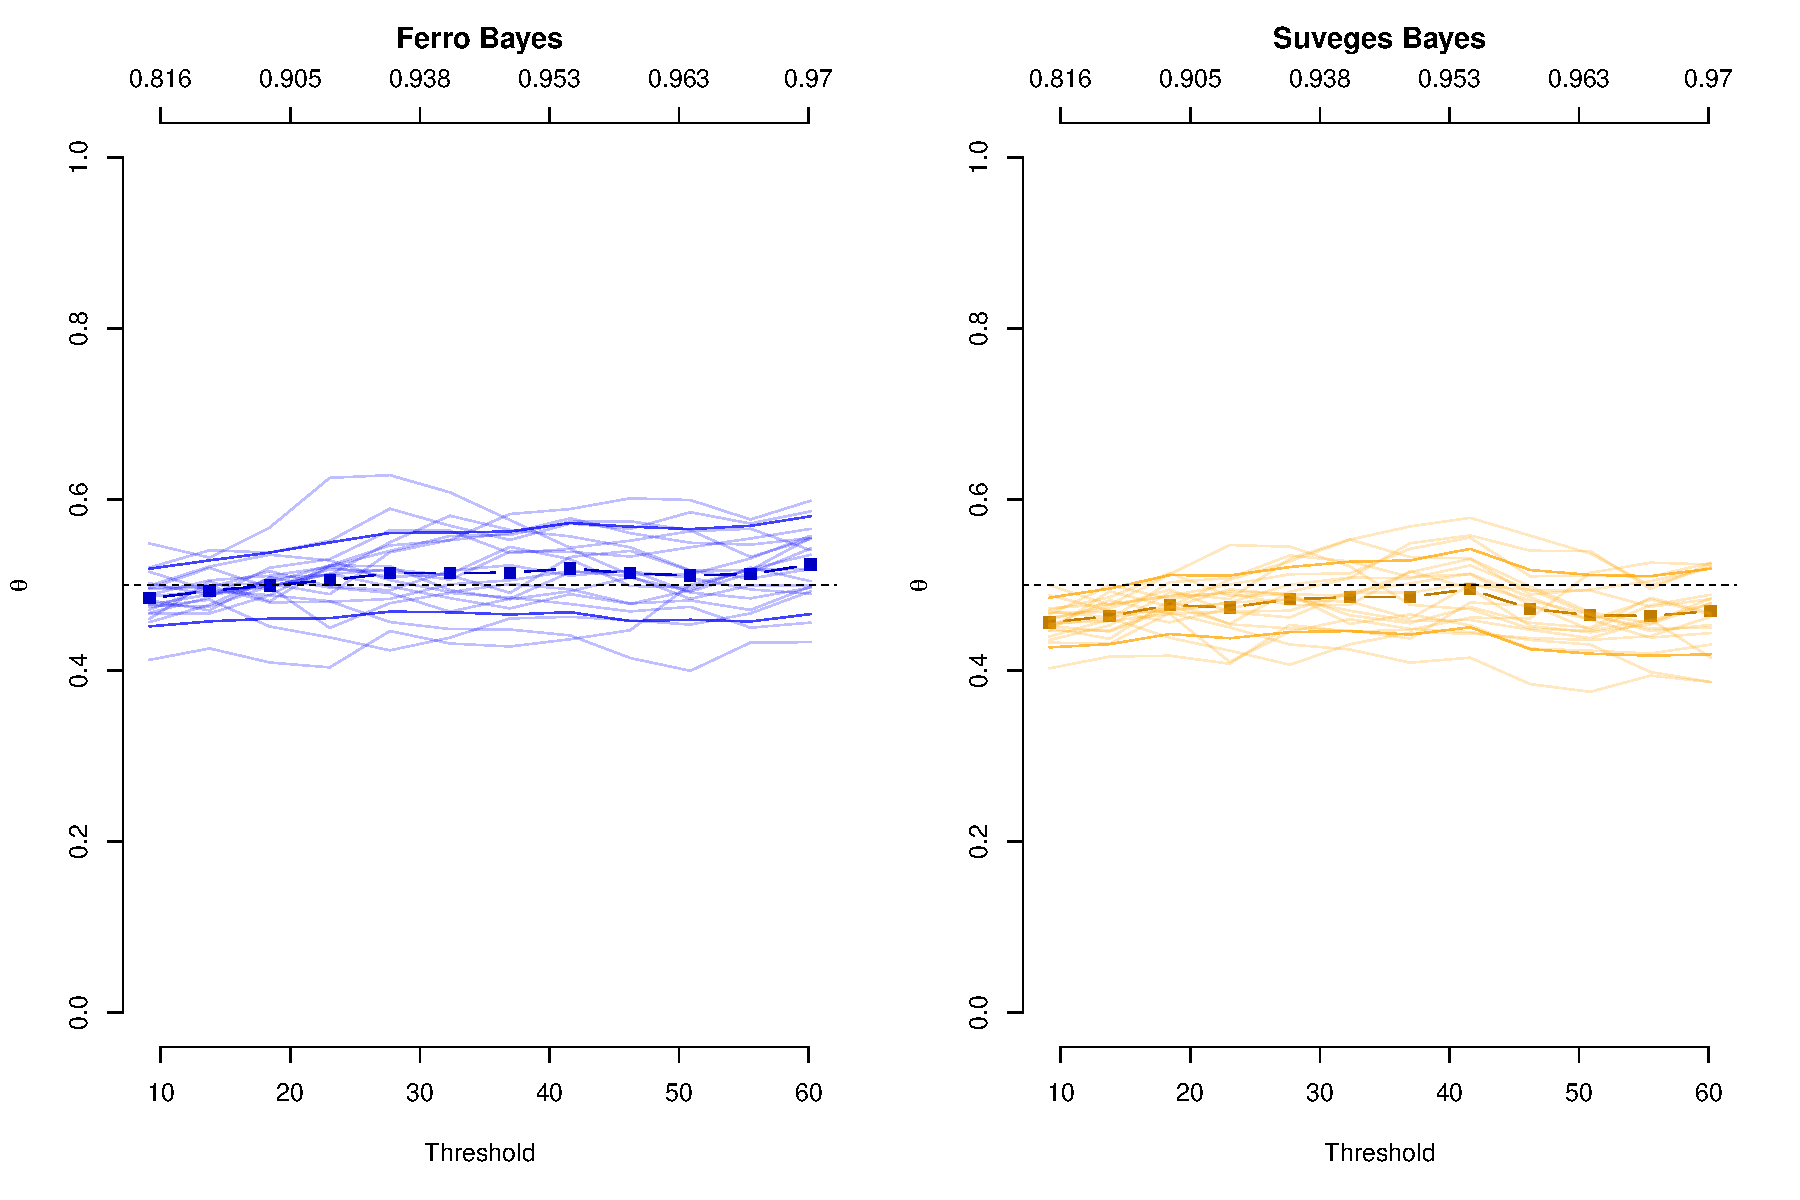
\includegraphics[width=5.5in, height=2.45in]{../extremal_comparison/figs/sim_frechet_hier_50_1000_20.pdf}
\caption{$\theta=0.50$, $n=1000$, $R=20$}
\end{center}
\end{figure}





\newpage

\begin{figure}
\begin{center}
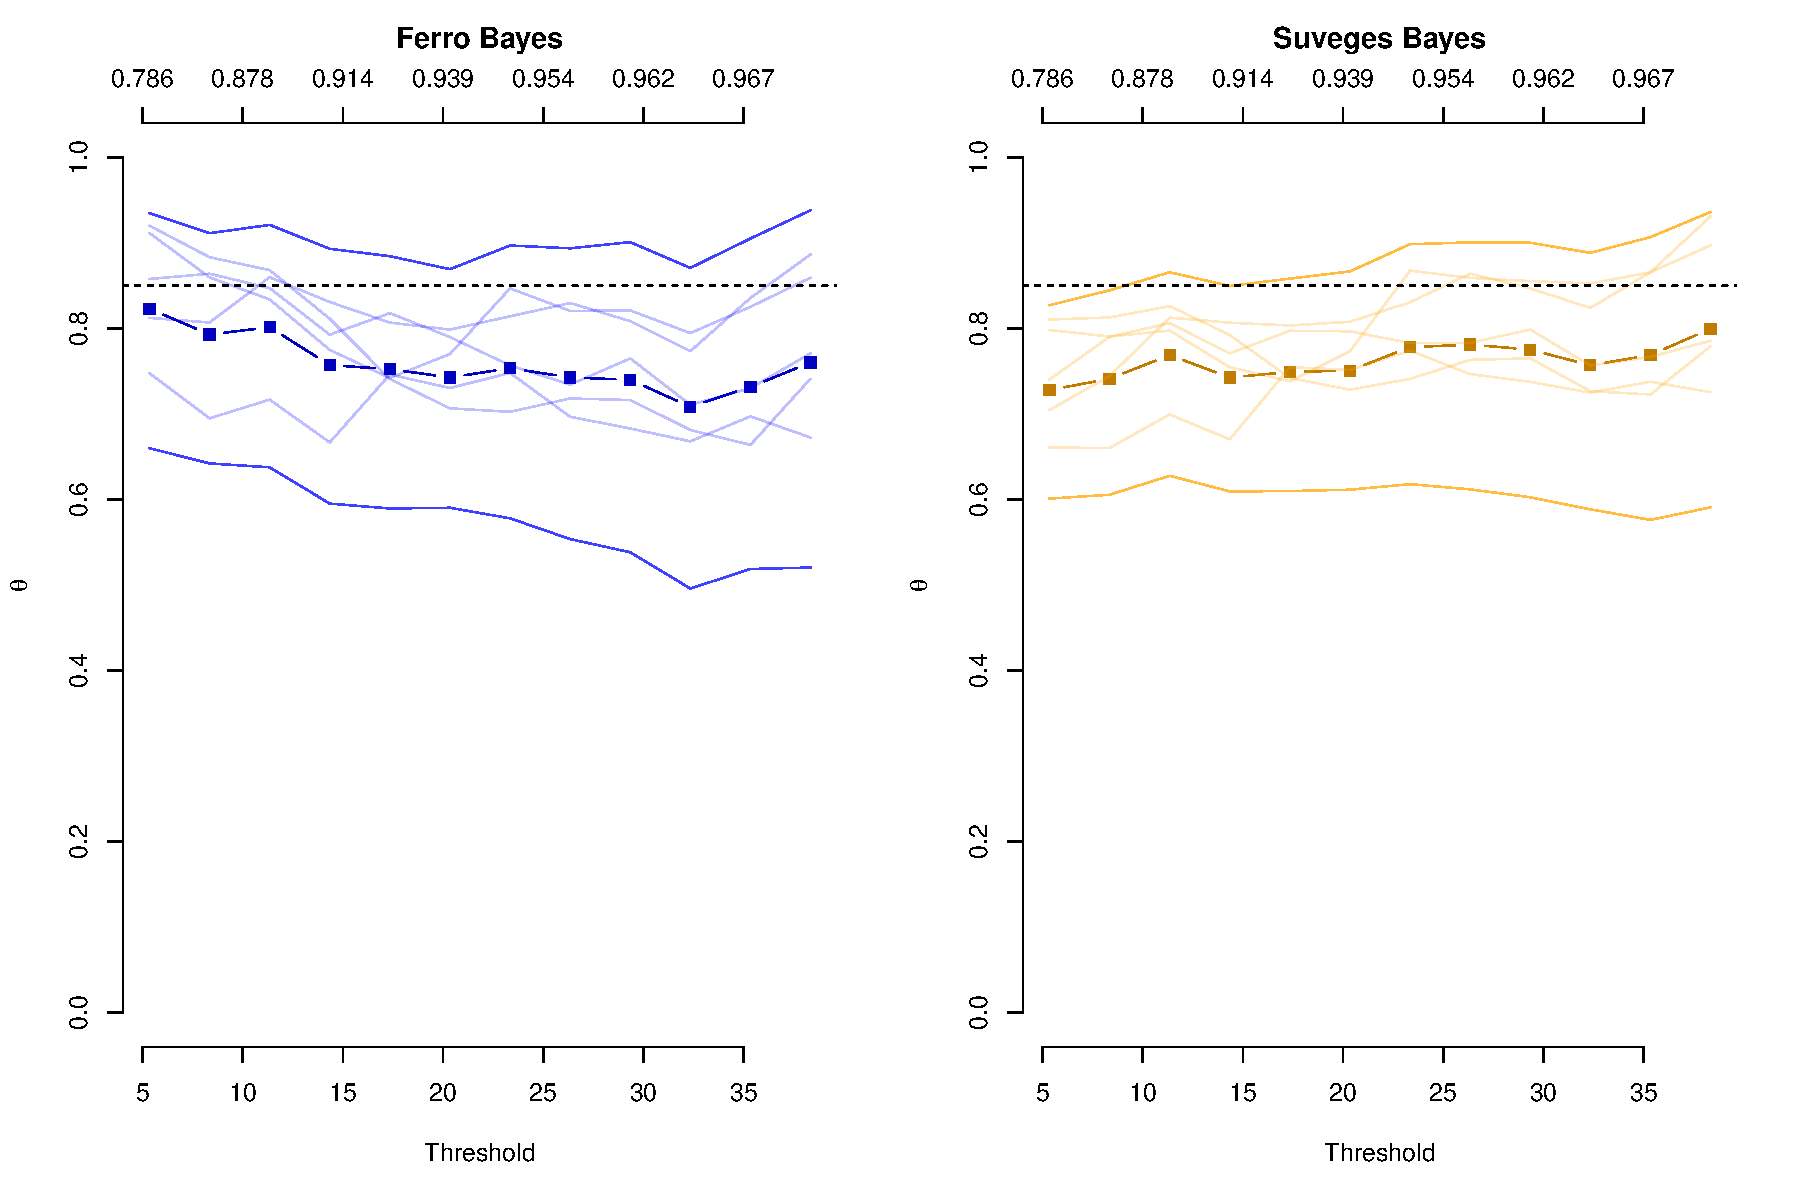
\includegraphics[width=5.5in, height=2.45in]{../extremal_comparison/figs/sim_frechet_hier_85_250_5.pdf}
\caption{$\theta=0.85$, $n=250$, $R=5$}
\end{center}
\end{figure}

\begin{figure}
\begin{center}
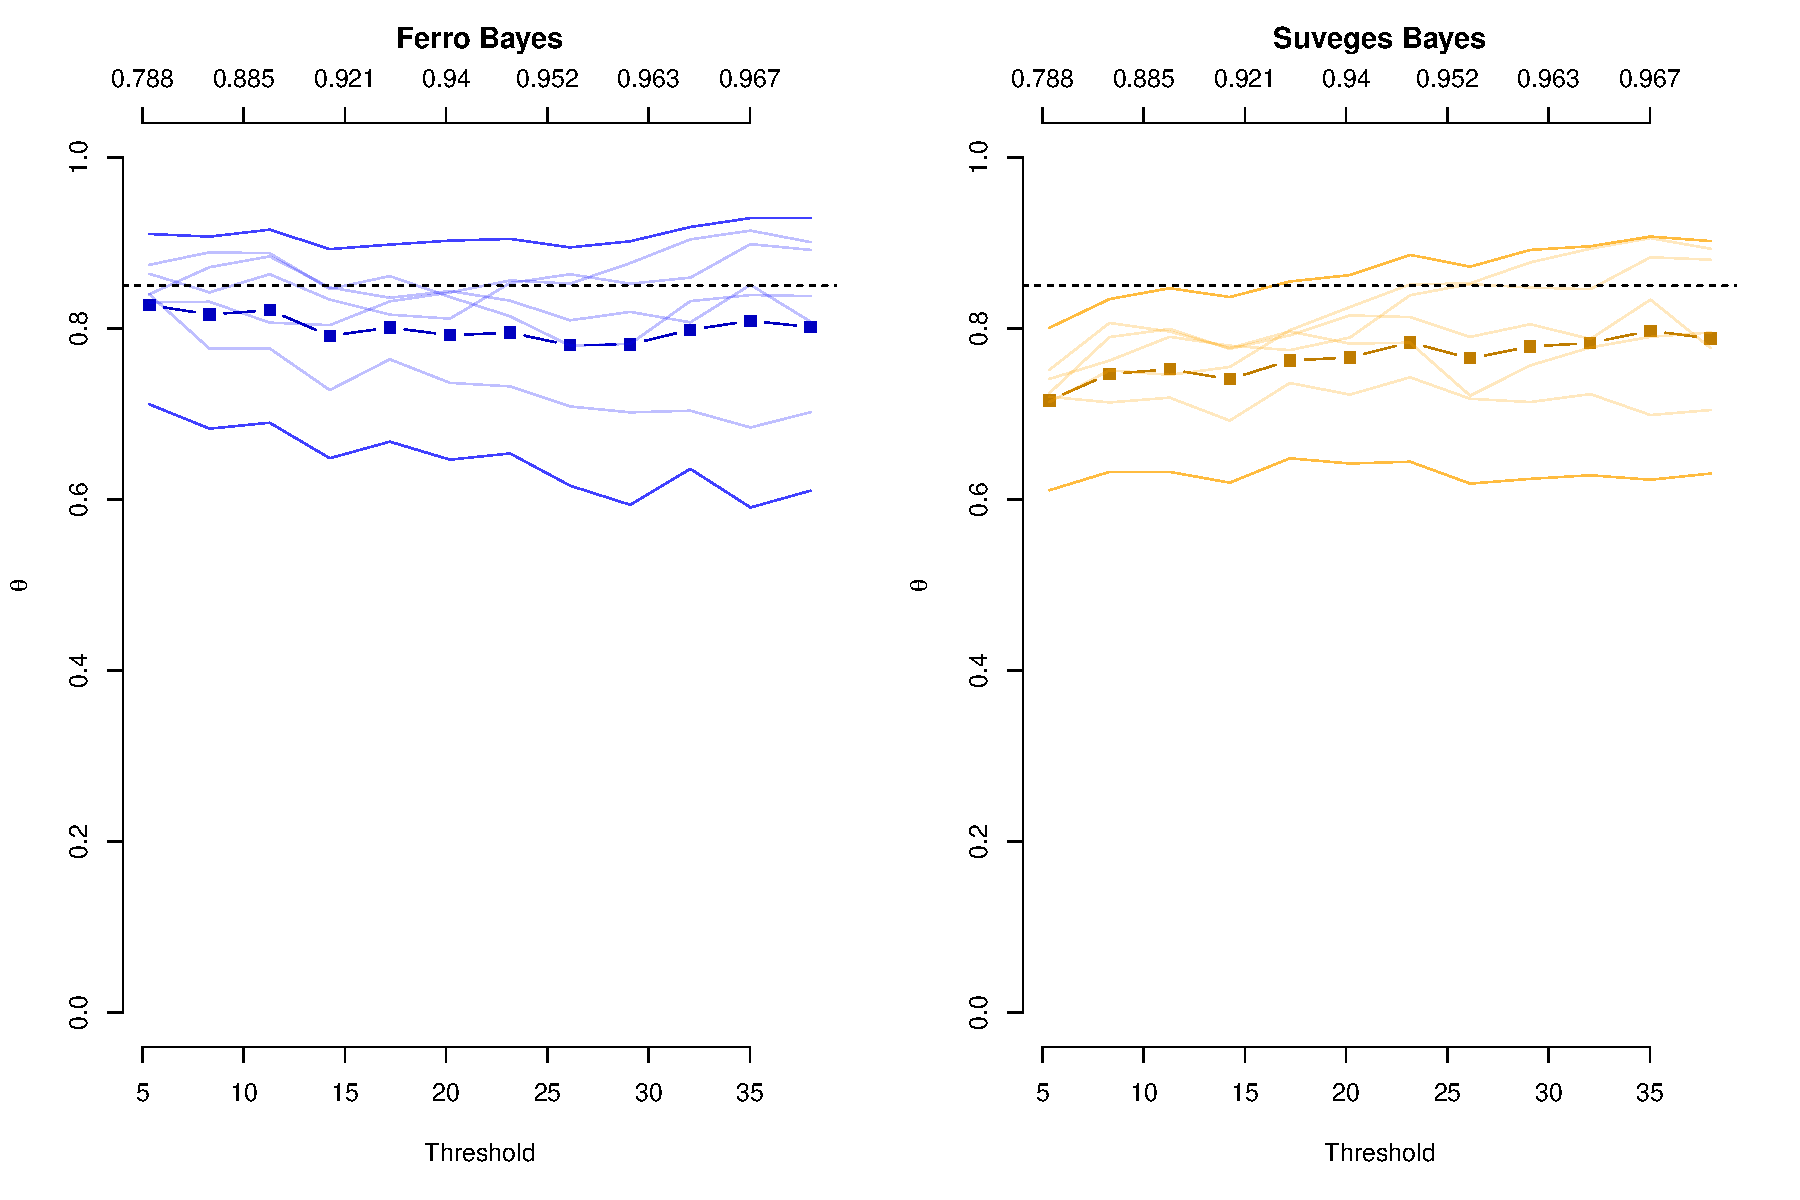
\includegraphics[width=5.5in, height=2.45in]{../extremal_comparison/figs/sim_frechet_hier_85_500_5.pdf}
\caption{$\theta=0.85$, $n=500$, $R=5$}
\end{center}
\end{figure}

\begin{figure}
\begin{center}
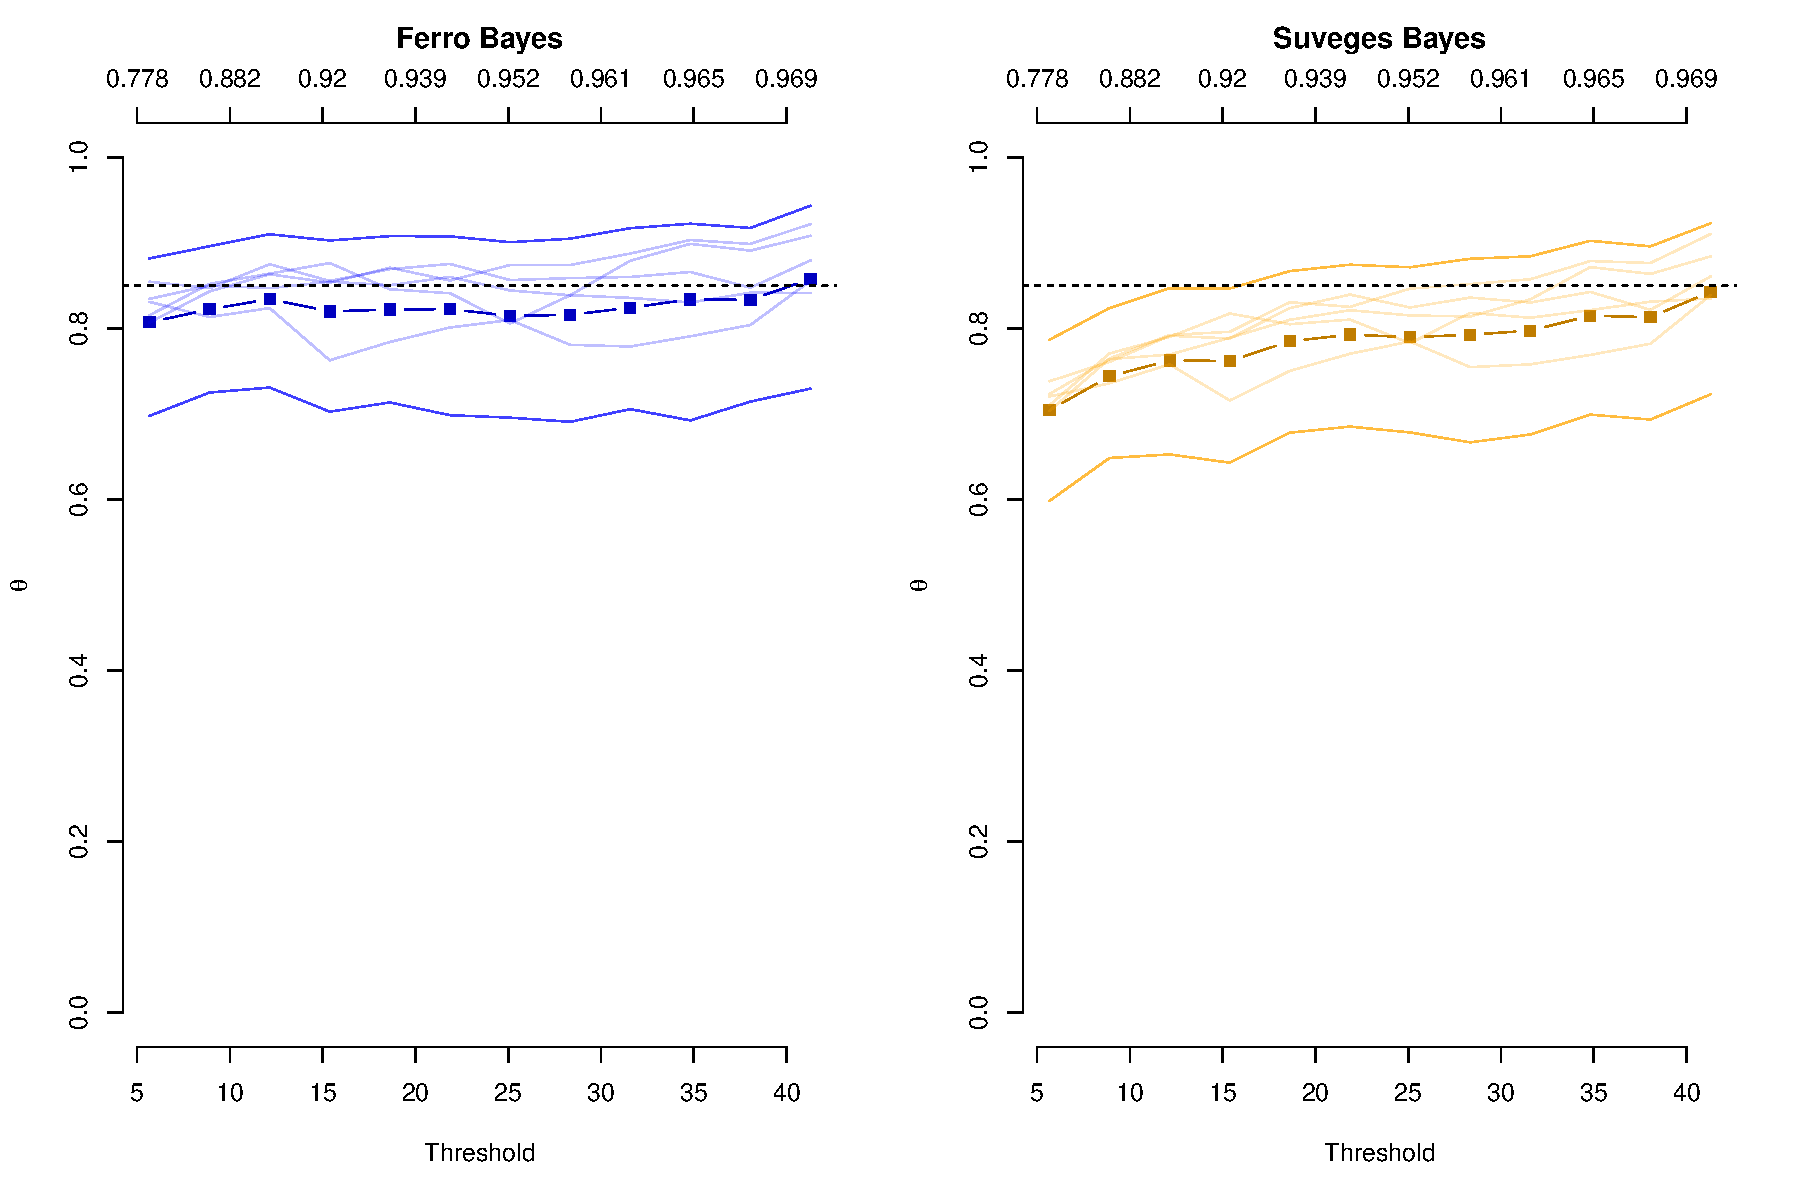
\includegraphics[width=5.5in, height=2.45in]{../extremal_comparison/figs/sim_frechet_hier_85_1000_5.pdf}
\caption{$\theta=0.85$, $n=1000$, $R=5$}
\end{center}
\end{figure}

\newpage

\begin{figure}
\begin{center}
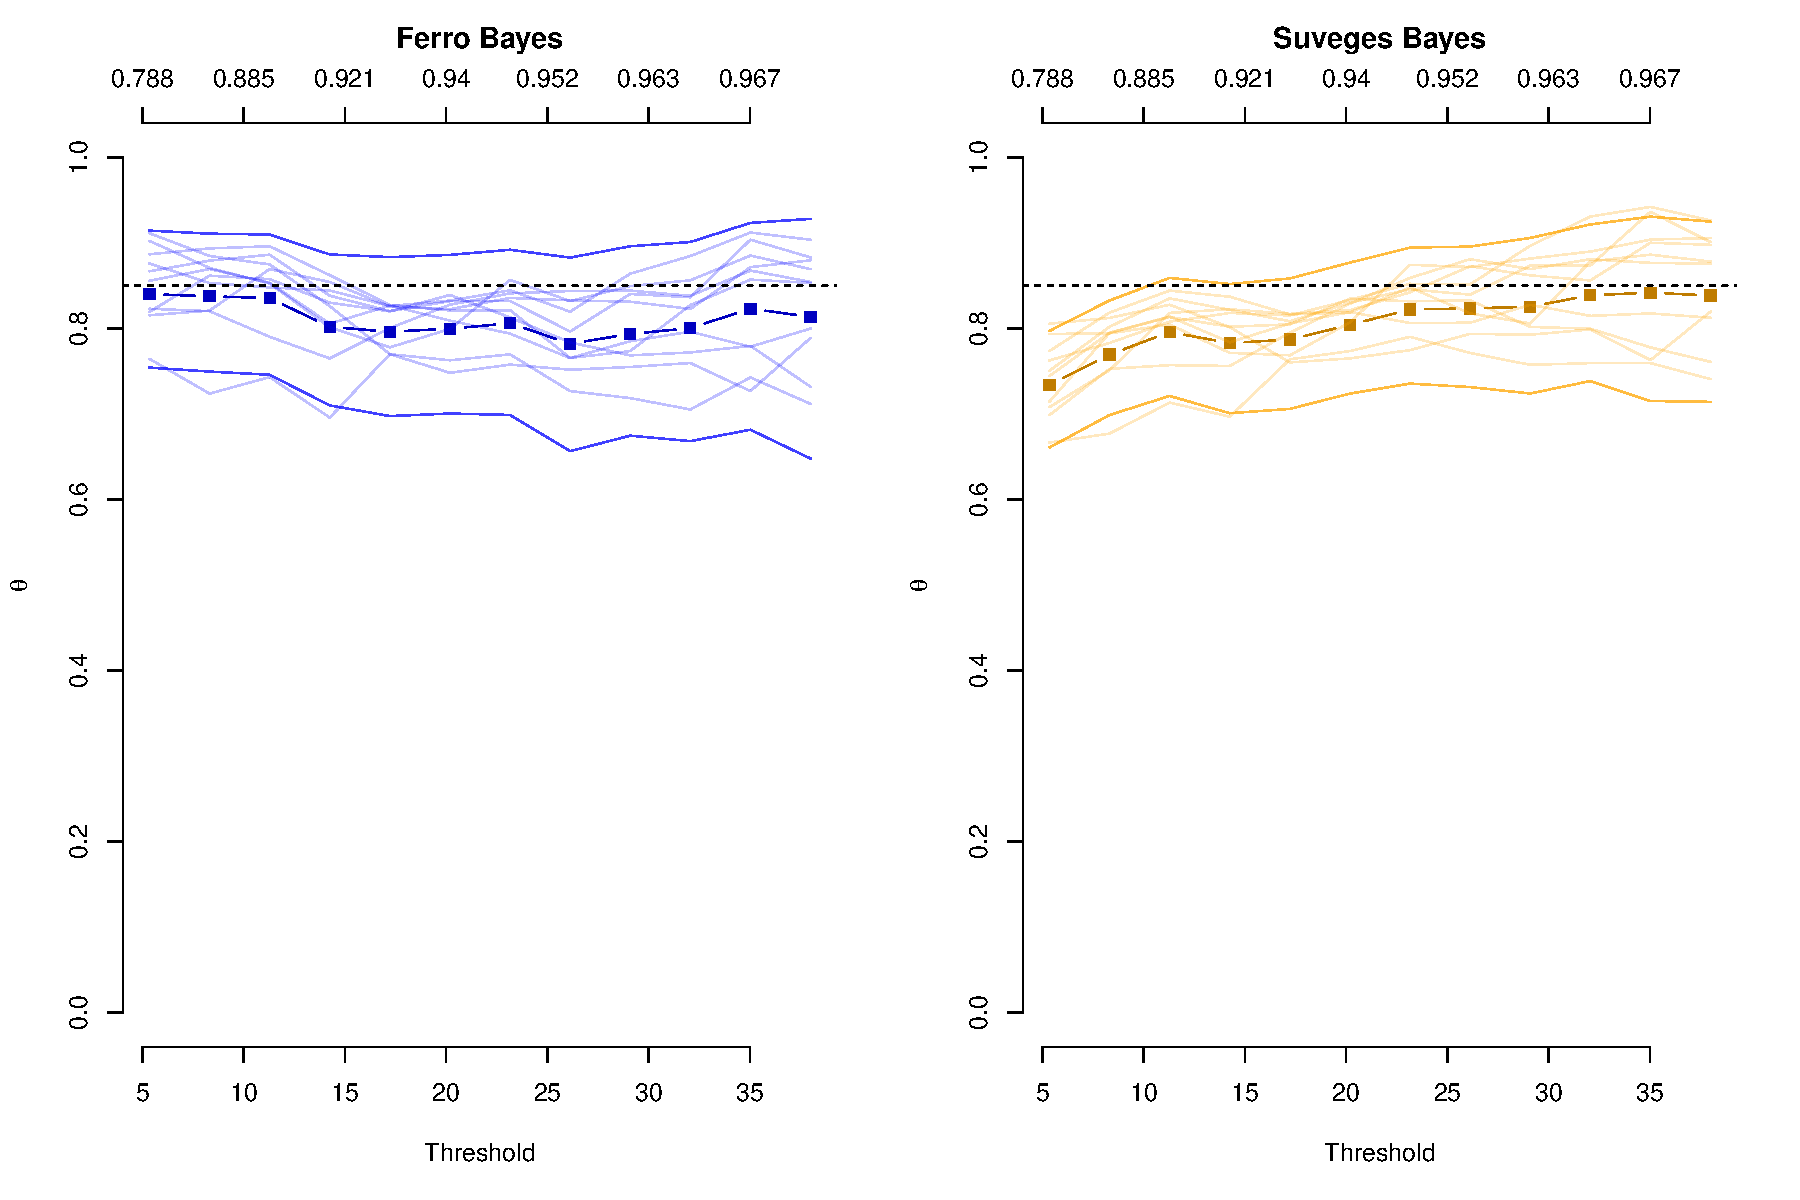
\includegraphics[width=5.5in, height=2.45in]{../extremal_comparison/figs/sim_frechet_hier_85_250_10.pdf}
\caption{$\theta=0.85$, $n=250$, $R=10$}
\end{center}
\end{figure}

\begin{figure}
\begin{center}
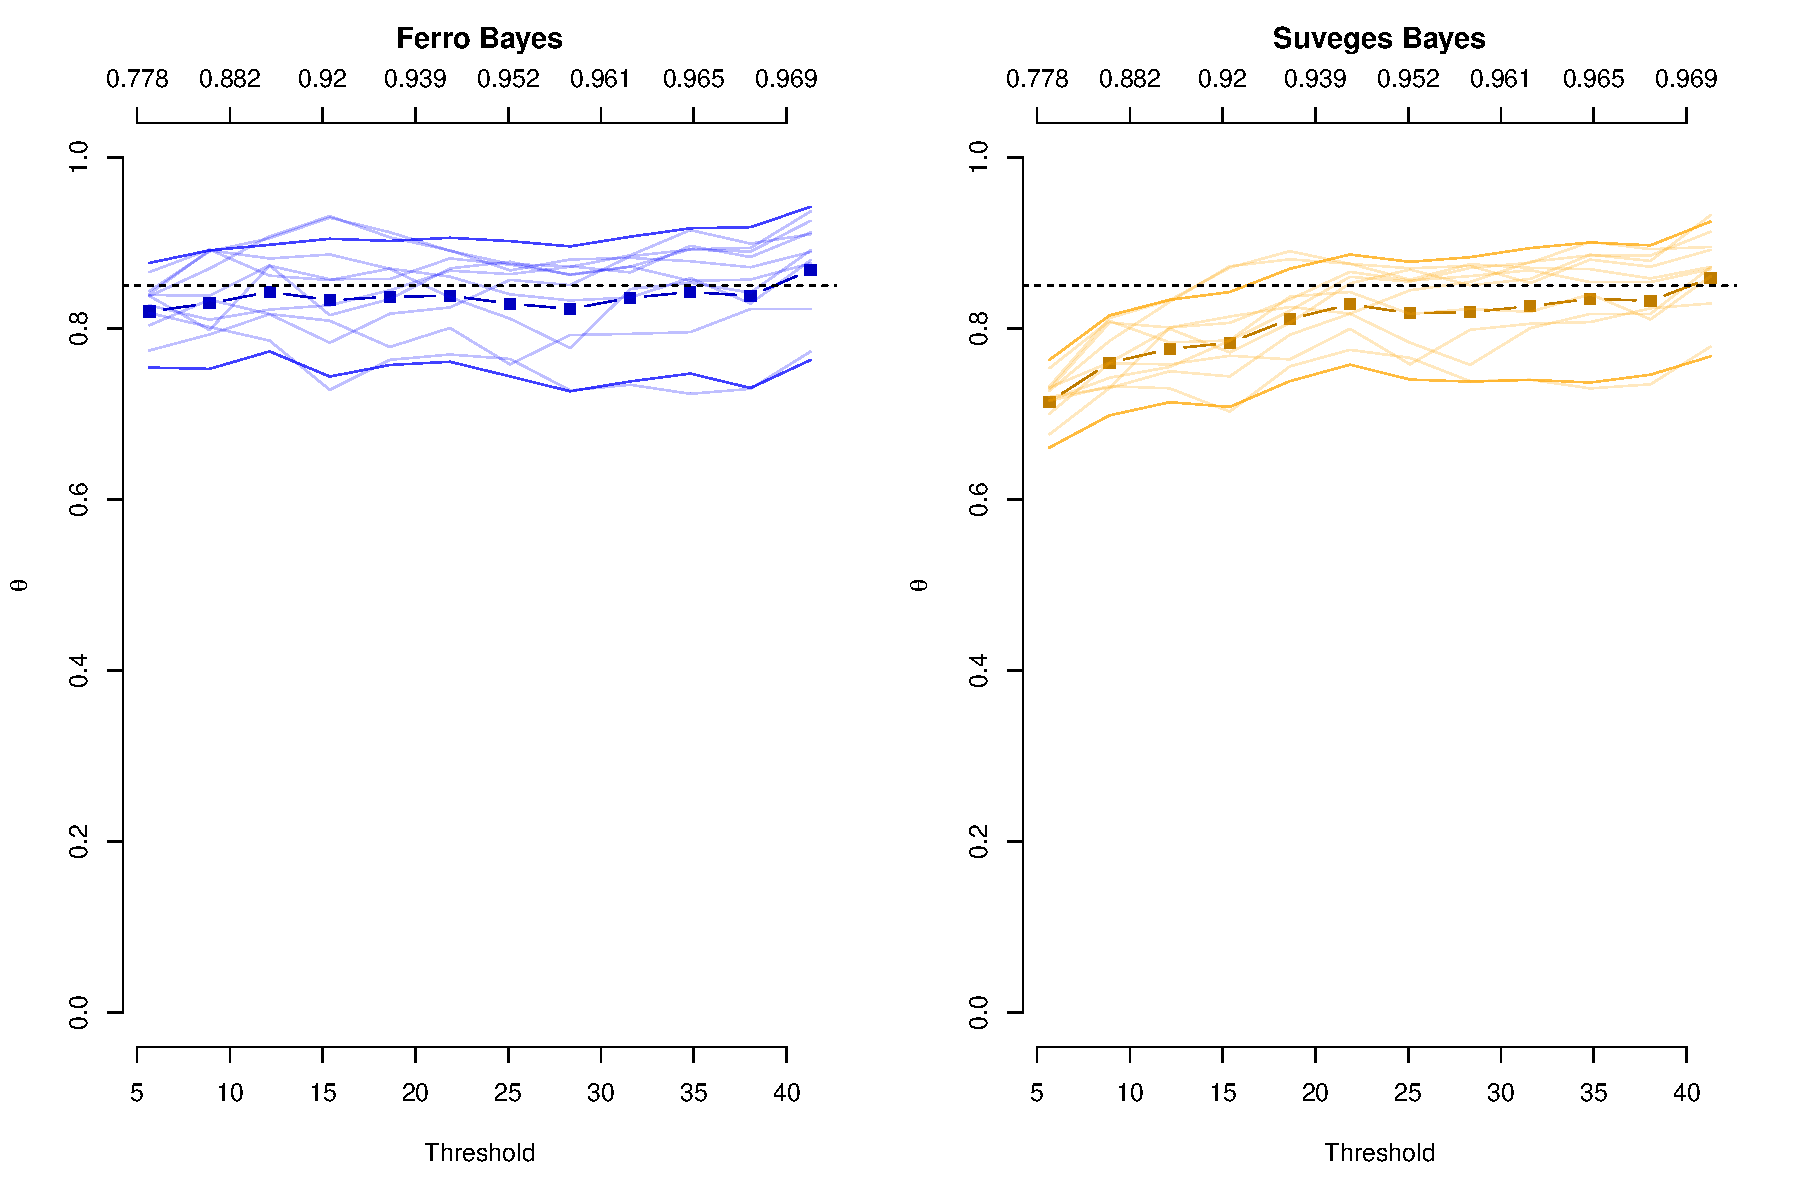
\includegraphics[width=5.5in, height=2.45in]{../extremal_comparison/figs/sim_frechet_hier_85_500_10.pdf}
\caption{$\theta=0.85$, $n=500$, $R=10$}
\end{center}
\end{figure}

\begin{figure}
\begin{center}
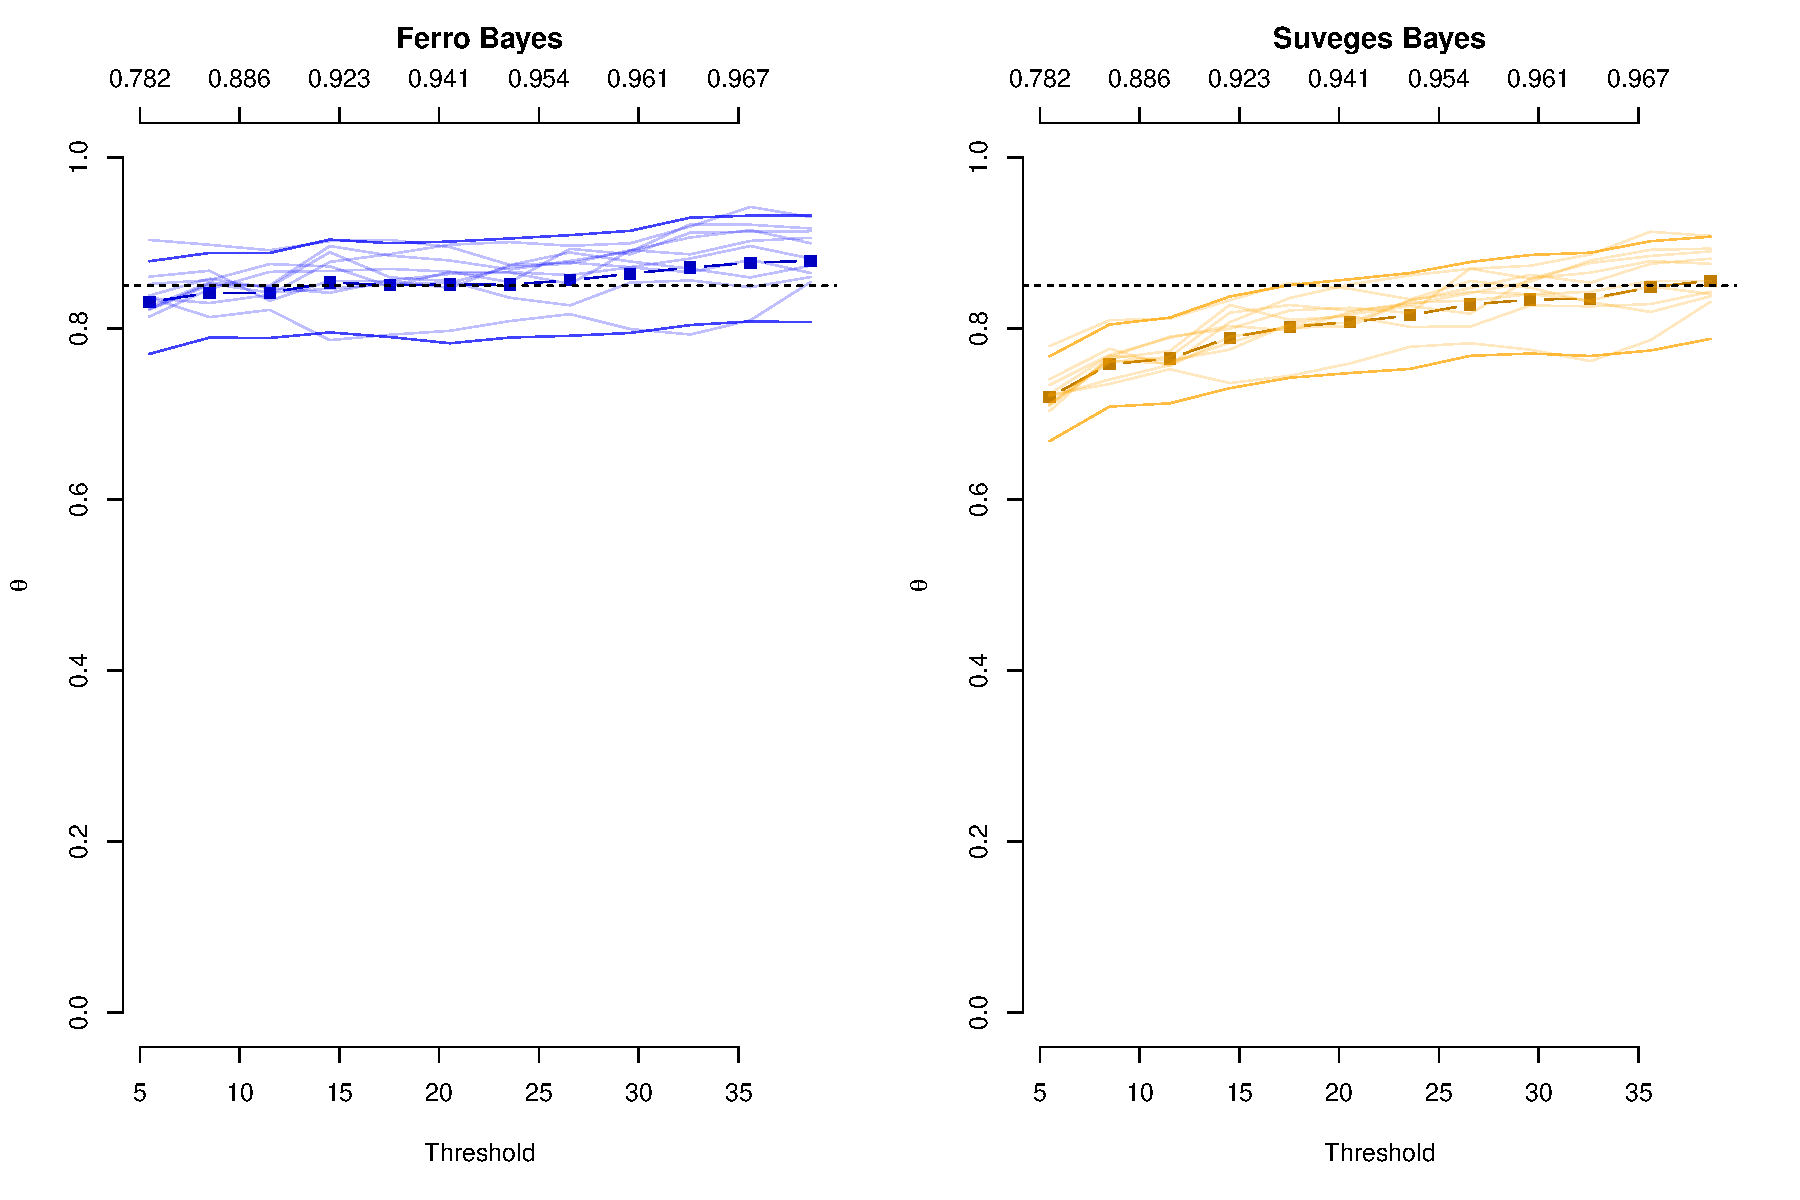
\includegraphics[width=5.5in, height=2.45in]{../extremal_comparison/figs/sim_frechet_hier_85_1000_10.pdf}
\caption{$\theta=0.85$, $n=1000$, $R=10$}
\end{center}
\end{figure}

\newpage

\begin{figure}
\begin{center}
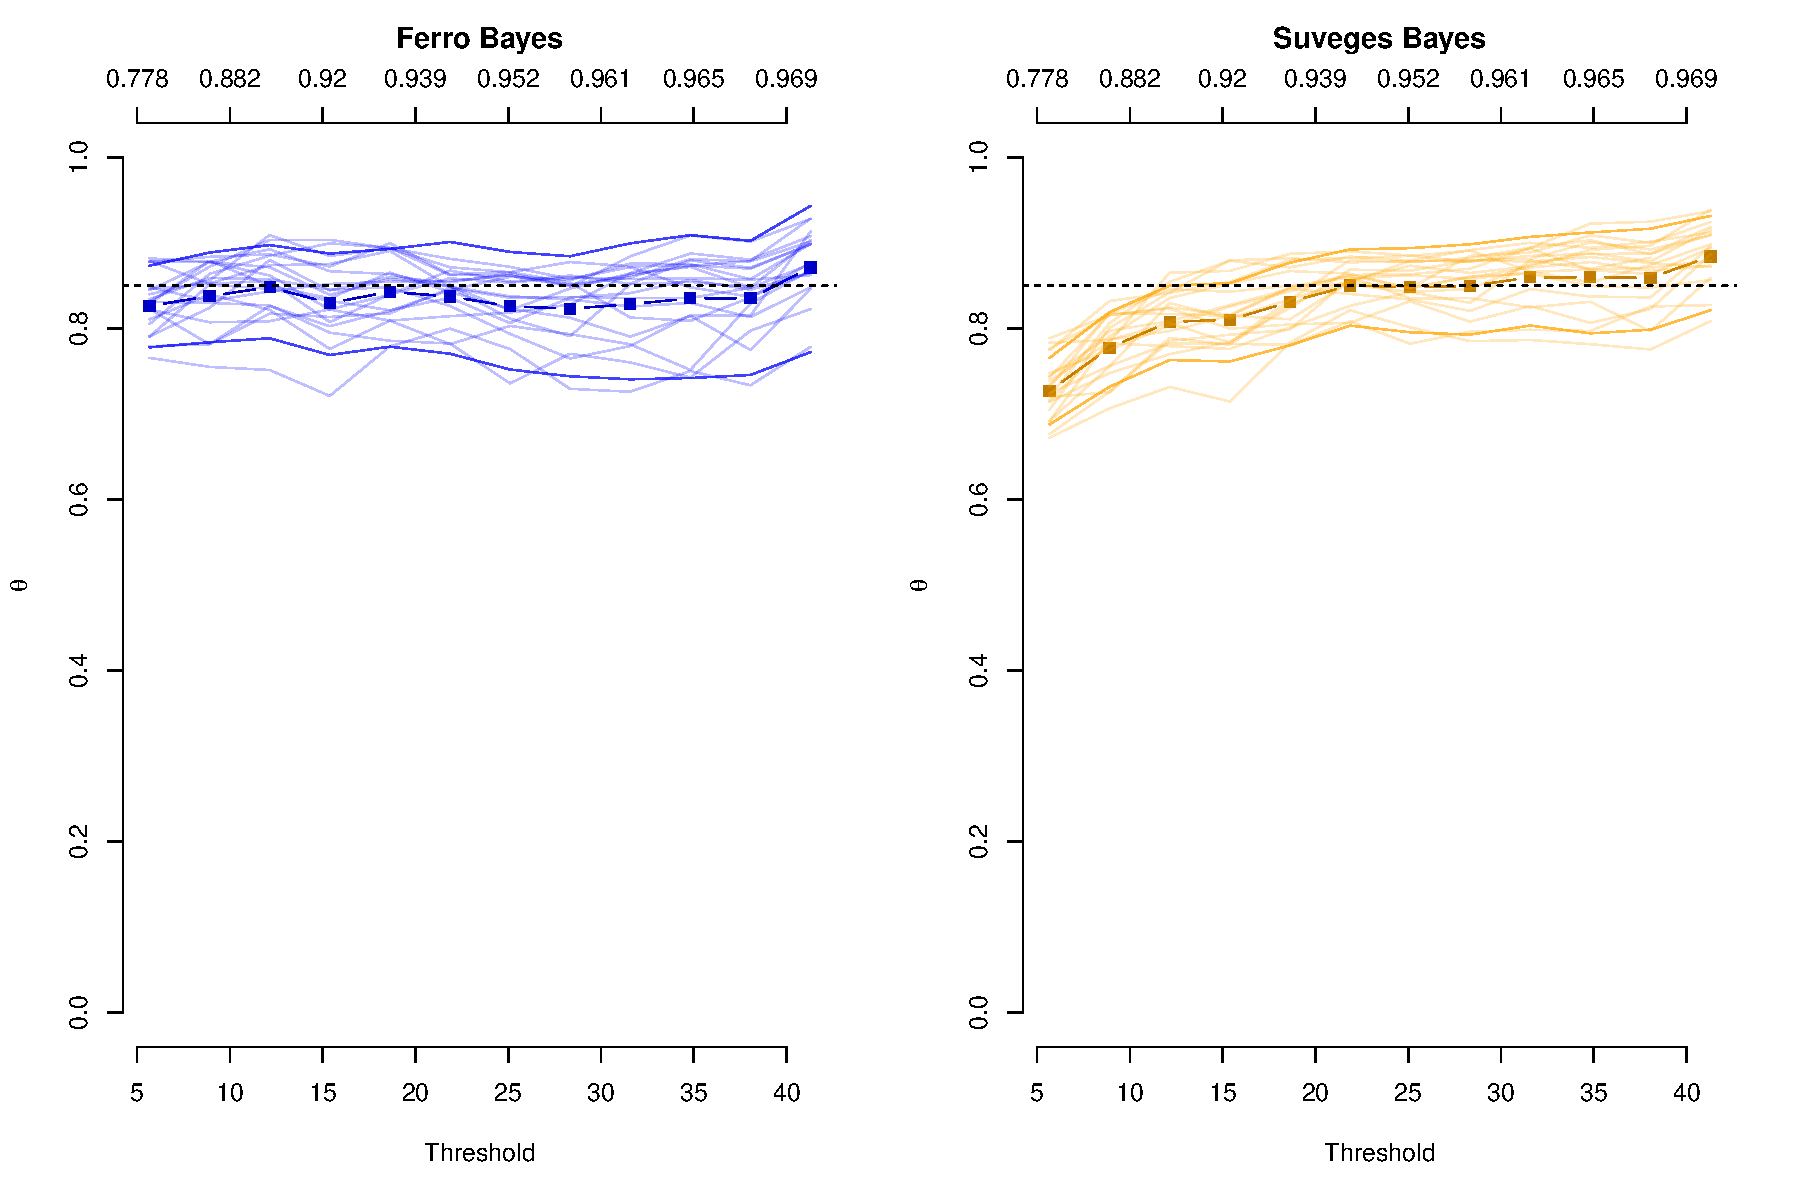
\includegraphics[width=5.5in, height=2.45in]{../extremal_comparison/figs/sim_frechet_hier_85_250_20.pdf}
\caption{$\theta=0.85$, $n=250$, $R=20$}
\end{center}
\end{figure}

\begin{figure}
\begin{center}
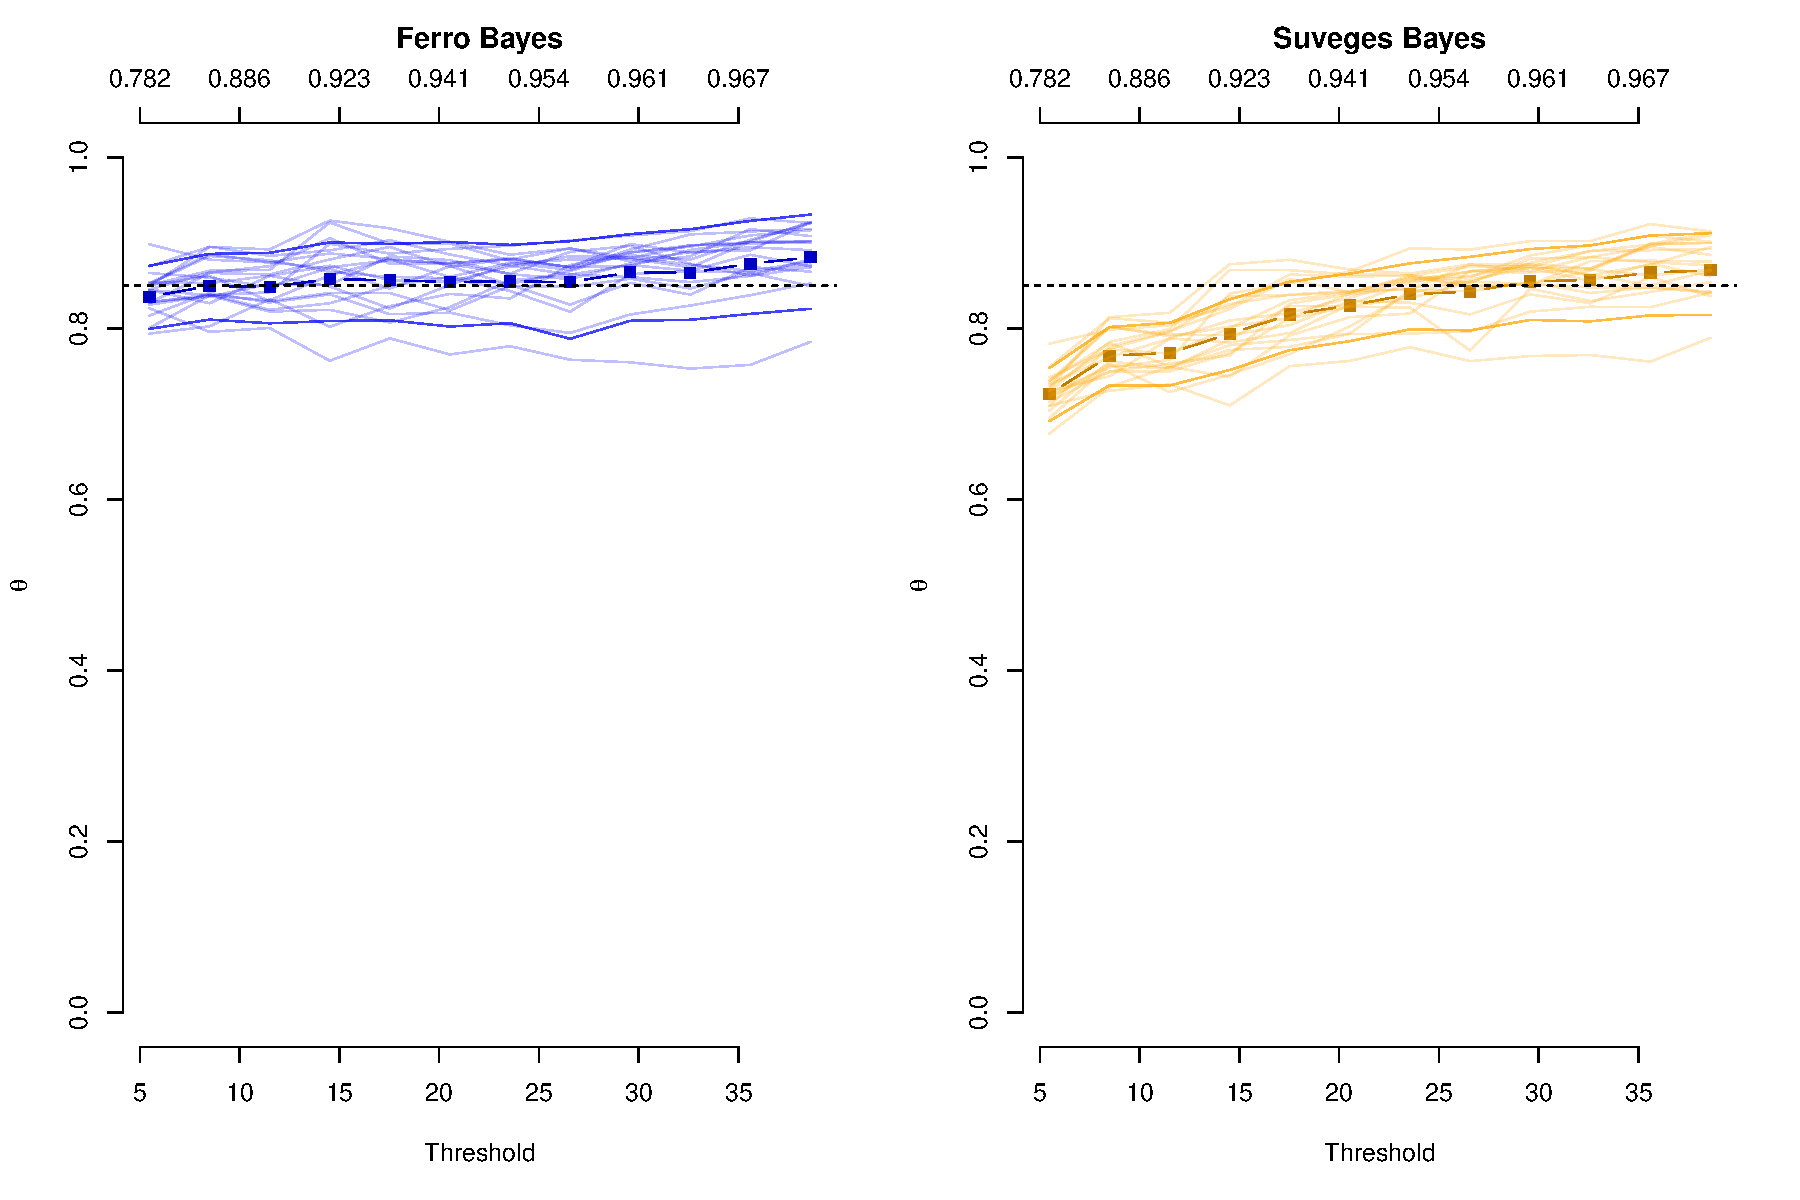
\includegraphics[width=5.5in, height=2.45in]{../extremal_comparison/figs/sim_frechet_hier_85_500_20.pdf}
\caption{$\theta=0.85$, $n=500$, $R=20$}
\end{center}
\end{figure}

\begin{figure}
\begin{center}
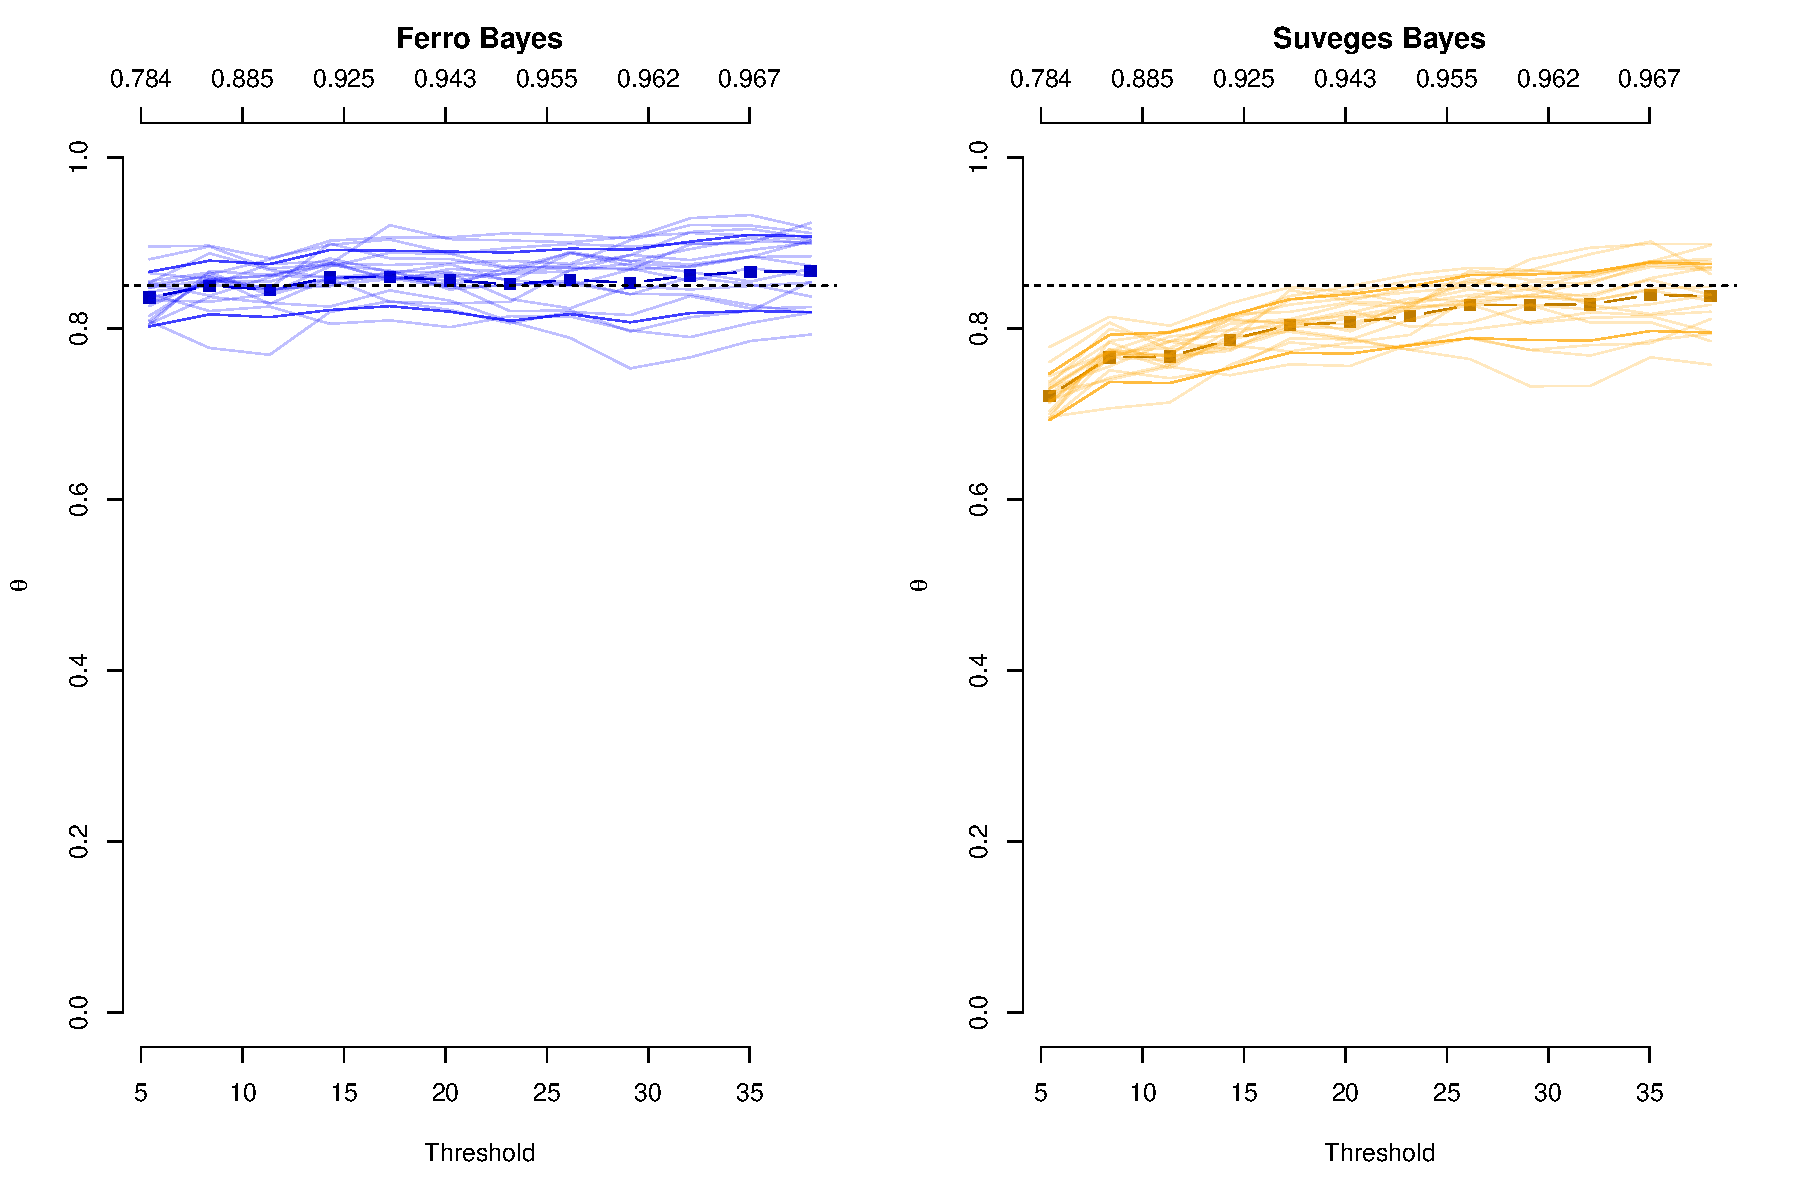
\includegraphics[width=5.5in, height=2.45in]{../extremal_comparison/figs/sim_frechet_hier_85_1000_20.pdf}
\caption{$\theta=0.85$, $n=1000$, $R=20$}
\end{center}
\end{figure}


\end{document}
